\documentclass[letterpaper, 10 pt, conference]{ieeeconf}
\IEEEoverridecommandlockouts
\overrideIEEEmargins
\pdfminorversion=4
% Colors:
% Blue-ish: 8FC2FF
% Yellow-ish: FFE599
% Red-ish: FF9999
% Brown-ish: E5C07B
% Blue/Green-ish: 397880

% Remove eventually
%\usepackage{showframe}
%\usepackage{lipsum}

\setcounter{secnumdepth}{3}
\usepackage{listings}
\usepackage{color}
\usepackage[hidelinks]{hyperref}
\let\proof\relax
\let\endproof\relax
\usepackage{amsmath}
\usepackage{amssymb}
\usepackage{amsthm}
\usepackage{subfig}
\usepackage{balance}
\usepackage{stfloats}
\usepackage{graphicx}
\usepackage{epstopdf}
\usepackage{bm}
\usepackage{booktabs}
\usepackage{array}
\usepackage{stfloats}
\usepackage{pdflscape}
\usepackage{pgfplots}
\usepackage{algorithm}
\usepackage{algorithmic}
\usepackage{setspace}
\usepackage{tikz}

%\usepackage[noadjust]{cite}
\usepackage{cite}

\renewcommand{\algorithmicrequire}{\textbf{Input:}}
\renewcommand{\algorithmicensure}{\textbf{Output:}}
\renewcommand\thealgorithm{\Roman{algorithm}}

% Italics for theorems
\theoremstyle{plain}
\newtheorem{theorem}{Theorem}
\renewcommand\thetheorem{\Roman{theorem}}

% Normal for all the rest
\newtheorem{lemma}{Lemma}
\renewcommand\thelemma{\Roman{lemma}}
\newtheorem{corollary}{Corollary}
\renewcommand\thecorollary{\Roman{corollary}}
\theoremstyle{definition}
\newtheorem{problem}{Problem}
\renewcommand\theproblem{\Roman{problem}}

% https://tex.stackexchange.com/questions/53978/custom-theorem-numbering
\newtheorem{innercustomprb}{Problem}
\newenvironment{customprb}[1]
  {\renewcommand\theinnercustomprb{#1}\innercustomprb}
  {\endinnercustomprb}

\newtheorem{innercustomhpt}{Hypothesis}
\newenvironment{customhpt}[1]
  {\renewcommand\theinnercustomhpt{#1}\innercustomhpt}
  {\endinnercustomhpt}

\newtheorem{innercustomobs}{Observation}
\newenvironment{customobs}[1]
  {\renewcommand\theinnercustomobs{#1}\innercustomobs}
  {\endinnercustomobs}

\newtheorem{innercustomcnj}{Conjecture}
\newenvironment{customcnj}[1]
  {\renewcommand\theinnercustomcnj{#1}\innercustomcnj}
  {\endinnercustomcnj}

\newtheorem{definition}{Definition}
\renewcommand\thedefinition{\Roman{definition}}
\newtheorem{remark}{Remark}
\renewcommand\theremark{\Roman{remark}}
\newtheorem{proposition}{Proposition}
\renewcommand\theproposition{\Roman{proposition}}
\newtheorem{objective}{Objective}
\renewcommand\theobjective{\Roman{objective}}
\newtheorem{operation}{Operation}
\renewcommand\theoperation{\Roman{operation}}

\renewcommand{\qedsymbol}{$\blacksquare$}

\definecolor{mygray}{rgb}{0.5,0.5,0.5}
\definecolor{keyword}{rgb}{0.5,0.5,0.5}
\definecolor{greenCode}{rgb}{0, 0.6, 0}

\lstdefinelanguage{HTTP}{
  keywords={GET},
  ndkeywords={PUT},
  comment=[s]{PO}{T},
  morecomment=[s]{D}{LETE}
}

\lstdefinestyle{customc}{
  belowcaptionskip=1\baselineskip,
  language={HTTP},
  breaklines=true,
  frame=tb,
  captionpos=b,
  keywordstyle=\bfseries\color{greenCode},
  ndkeywordstyle=\bfseries\color{red},
  commentstyle=\bfseries\color{magenta},
  stringstyle=\bfseries\color{black},
  xleftmargin={0.75cm},
  showstringspaces=false,
  basicstyle=\footnotesize\ttfamily,
  numbers=left,
  numberstyle=\small\color{black},
}

\lstset{escapechar=@,style=customc}

%\ifCLASSINFOpdf
   %\usepackage[pdftex]{graphicx}
%\else
%\fi

\usepackage{flushend} % Equalize last page
\usepackage[colorinlistoftodos]{todonotes}

\usepackage{framed}

% Manipulate vspace for algorithm
\makeatletter
\newcommand\fs@spaceruled{\def\@fs@cfont{\bfseries}\let\@fs@capt\floatc@ruled
  \def\@fs@pre{\vspace{0.5\baselineskip}\hrule height.8pt depth0pt \kern2pt}%
  \def\@fs@post{\kern2pt\hrule\relax}%
  \def\@fs@mid{\kern2pt\hrule\kern2pt}%
  \let\@fs@iftopcapt\iftrue}
\makeatother


% Highlight algorithm parts with color
\newcommand*{\tikzmk}[1]{\tikz[remember picture,overlay,] \node (#1) {};\ignorespaces}
%define a boxing command, argument = colour of box
\newcommand{\boxit}[1]{\tikz[remember picture,overlay]{\node[yshift=3pt,fill=#1,opacity=.25,fit={($(A)+(-0.038\linewidth,.3\baselineskip)$)($(B)+(.9\linewidth,-.3\baselineskip)$)}] {};}\ignorespaces}


\begin{document}

\title{\LARGE \bf CBGL: Fast Monte Carlo Passive Global Localisation \\ for 2D LIDAR sensors}


\author{Alexandros Filotheou% <-this % stops a space
  \thanks{}
}

\maketitle
\thispagestyle{empty}
\pagestyle{empty}


%%%%%%%%%%%%%%%%%%%%%%%%%%%%%%%%%%%%%%%%%%%%%%%%%%%%%%%%%%%%%%%%%%%%%%%%%%%%%%%%
\begin{abstract}
  Navigation of a mobile robot is conditioned on the knowledge of its pose. In
observer-based localisation configurations its initial pose may not be knowable
in advance, leading to the need of its estimation. The Monte Carlo class of
solutions disperse hypotheses in the environment's map, which gradually
converge on an estimate. These methods are robust against noise but require
motion and time, which may be economised on. Feature-based solutions require
minimal estimation time but assume environmental structure, may be sensitive to
noise, and require preprocessing and tuning. The method proposed in this
article retains the positive qualities of the two main approaches to global
localisation and avoids their pitfalls: it requires a single measurement from a
2D LIDAR sensor, assumes no motion, environmental structure, or parameter
tuning in a per-environment or sensor basis, and is robust against noise.  A
large number of tests, in real and simulated conditions, involving disparate
environments and sensor properties, illustrate that the proposed method
outperforms state-of-the-art methods of both classes in terms of pose discovery
rate and execution time. The source code is available for download.

\end{abstract}

\begin{keywords}
global localisation, 2D LIDAR, monte carlo, scan--to--map-scan matching
\end{keywords}

%%%%%%%%%%%%%%%%%%%%%%%%%%%%%%%%%%%%%%%%%%%%%%%%%%%%%%%%%%%%%%%%%%%%%%%%%%%%%%%%
\section{Introduction}
  This paper addresses the problem of Passive Global Localisation of a 2D LIDAR
sensor, i.e. the estimation of its location and orientation within a given map,
under complete locational and orientational uncertainty, without prescribing
motion commands (to the mobile robot that the sensor is assumed mounted to) for
further knowledge acquisition. Specifically the problem is formalised in
Problem \ref{prob:the_problem}:

%%%%%%%%%%%%%%%%%%%%%%%%%%%%%%%%%%%%%%%%%%%%%%%%%%%%%%%%%%%%%%%%%%%%%%%%%%%%%%%%
\begin{customprb}{P}
  \label{prob:the_problem}
  Let the unknown pose of an immobile 2D range sensor whose angular range is
  $\lambda$ be $\bm{p}(\bm{l},\theta)$, $\bm{l} = (x,y)$, with respect to the
  reference frame of map $\bm{M}$. Let the range sensor measure range scan
  $\mathcal{S}_R$. The objective is the estimation of $\bm{p}$ given $\bm{M}$,
  $\lambda$, and $\mathcal{S}_R$.
\end{customprb}
%%%%%%%%%%%%%%%%%%%%%%%%%%%%%%%%%%%%%%%%%%%%%%%%%%%%%%%%%%%%%%%%%%%%%%%%%%%%%%%%

\begin{figure}\vspace{0.4em}
  \subfloat{% GNUPLOT: LaTeX picture with Postscript
\begingroup
  \makeatletter
  \providecommand\color[2][]{%
    \GenericError{(gnuplot) \space\space\space\@spaces}{%
      Package color not loaded in conjunction with
      terminal option `colourtext'%
    }{See the gnuplot documentation for explanation.%
    }{Either use 'blacktext' in gnuplot or load the package
      color.sty in LaTeX.}%
    \renewcommand\color[2][]{}%
  }%
  \providecommand\includegraphics[2][]{%
    \GenericError{(gnuplot) \space\space\space\@spaces}{%
      Package graphicx or graphics not loaded%
    }{See the gnuplot documentation for explanation.%
    }{The gnuplot epslatex terminal needs graphicx.sty or graphics.sty.}%
    \renewcommand\includegraphics[2][]{}%
  }%
  \providecommand\rotatebox[2]{#2}%
  \@ifundefined{ifGPcolor}{%
    \newif\ifGPcolor
    \GPcolorfalse
  }{}%
  \@ifundefined{ifGPblacktext}{%
    \newif\ifGPblacktext
    \GPblacktexttrue
  }{}%
  % define a \g@addto@macro without @ in the name:
  \let\gplgaddtomacro\g@addto@macro
  % define empty templates for all commands taking text:
  \gdef\gplfronttext{}%
  \gdef\gplfronttext{}%
  \makeatother
  \ifGPblacktext
    % no textcolor at all
    \def\colorrgb#1{}%
    \def\colorgray#1{}%
  \else
    % gray or color?
    \ifGPcolor
      \def\colorrgb#1{\color[rgb]{#1}}%
      \def\colorgray#1{\color[gray]{#1}}%
      \expandafter\def\csname LTw\endcsname{\color{white}}%
      \expandafter\def\csname LTb\endcsname{\color{black}}%
      \expandafter\def\csname LTa\endcsname{\color{black}}%
      \expandafter\def\csname LT0\endcsname{\color[rgb]{1,0,0}}%
      \expandafter\def\csname LT1\endcsname{\color[rgb]{0,1,0}}%
      \expandafter\def\csname LT2\endcsname{\color[rgb]{0,0,1}}%
      \expandafter\def\csname LT3\endcsname{\color[rgb]{1,0,1}}%
      \expandafter\def\csname LT4\endcsname{\color[rgb]{0,1,1}}%
      \expandafter\def\csname LT5\endcsname{\color[rgb]{1,1,0}}%
      \expandafter\def\csname LT6\endcsname{\color[rgb]{0,0,0}}%
      \expandafter\def\csname LT7\endcsname{\color[rgb]{1,0.3,0}}%
      \expandafter\def\csname LT8\endcsname{\color[rgb]{0.5,0.5,0.5}}%
    \else
      % gray
      \def\colorrgb#1{\color{black}}%
      \def\colorgray#1{\color[gray]{#1}}%
      \expandafter\def\csname LTw\endcsname{\color{white}}%
      \expandafter\def\csname LTb\endcsname{\color{black}}%
      \expandafter\def\csname LTa\endcsname{\color{black}}%
      \expandafter\def\csname LT0\endcsname{\color{black}}%
      \expandafter\def\csname LT1\endcsname{\color{black}}%
      \expandafter\def\csname LT2\endcsname{\color{black}}%
      \expandafter\def\csname LT3\endcsname{\color{black}}%
      \expandafter\def\csname LT4\endcsname{\color{black}}%
      \expandafter\def\csname LT5\endcsname{\color{black}}%
      \expandafter\def\csname LT6\endcsname{\color{black}}%
      \expandafter\def\csname LT7\endcsname{\color{black}}%
      \expandafter\def\csname LT8\endcsname{\color{black}}%
    \fi
  \fi
    \setlength{\unitlength}{0.0500bp}%
    \ifx\gptboxheight\undefined%
      \newlength{\gptboxheight}%
      \newlength{\gptboxwidth}%
      \newsavebox{\gptboxtext}%
    \fi%
    \setlength{\fboxrule}{0.5pt}%
    \setlength{\fboxsep}{1pt}%
\begin{picture}(5000.00,3000.00)%
    \gplgaddtomacro\gplfronttext{%
    }%
    \gplgaddtomacro\gplfronttext{%
    }%
    \gplgaddtomacro\gplfronttext{%
    }%
    \gplgaddtomacro\gplfronttext{%
      \colorrgb{0.15,0.15,0.15}%
      \put(475,1279){\makebox(0,0)[r]{\strut{}$0$}}%
      \colorrgb{0.15,0.15,0.15}%
      %\put(791,1256){\makebox(0,0)[r]{\strut{}$5$}}%
      \colorrgb{0.15,0.15,0.15}%
      \put(1107,1233){\makebox(0,0)[r]{\strut{}$10$}}%
      \colorrgb{0.15,0.15,0.15}%
      %\put(1424,1209){\makebox(0,0)[r]{\strut{}$15$}}%
      \colorrgb{0.15,0.15,0.15}%
      \put(1740,1186){\makebox(0,0)[r]{\strut{}$20$}}%
      \colorrgb{0.15,0.15,0.15}%
      %\put(2056,1163){\makebox(0,0)[r]{\strut{}$25$}}%
      \colorrgb{0.15,0.15,0.15}%
      \put(2373,1140){\makebox(0,0)[r]{\strut{}$30$}}%
      \colorrgb{0.15,0.15,0.15}%
      %\put(2688,1117){\makebox(0,0)[r]{\strut{}$35$}}%
      \colorrgb{0.15,0.15,0.15}%
      \put(3004,1094){\makebox(0,0)[r]{\strut{}$40$}}%
      \colorrgb{0.15,0.15,0.15}%
      \put(3528,1236){\makebox(0,0)[l]{\strut{}$0$}}%
      \colorrgb{0.15,0.15,0.15}%
      %\put(3764,1366){\makebox(0,0)[l]{\strut{}$5$}}%
      \colorrgb{0.15,0.15,0.15}%
      \put(4000,1496){\makebox(0,0)[l]{\strut{}$10$}}%
      \colorrgb{0.15,0.15,0.15}%
      %\put(4236,1626){\makebox(0,0)[l]{\strut{}$15$}}%
      \colorrgb{0.15,0.15,0.15}%
      \put(4471,1756){\makebox(0,0)[l]{\strut{}$20$}}%
      \colorrgb{0.15,0.15,0.15}%
      \put(473,2125){\makebox(0,0)[r]{\strut{}$0.0$}}%
      \colorrgb{0.15,0.15,0.15}%
      \put(473,1817){\makebox(0,0)[r]{\strut{}$2.0$}}%
      \colorrgb{0.15,0.15,0.15}%
      \put(473,1509){\makebox(0,0)[r]{\strut{}$4.0$}}%
    }%
    \put(0,0){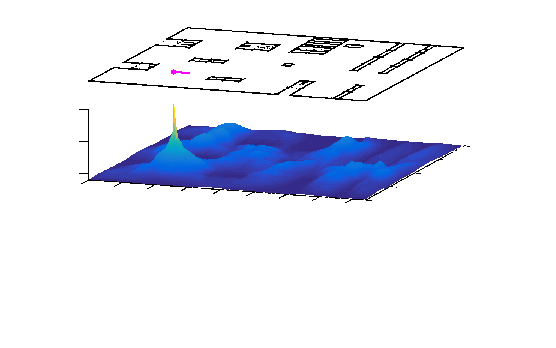
\includegraphics{./figures/face_top}}%
    \gplfronttext
  \end{picture}%
\endgroup
    \label{fig:a}} \vspace{-1.7cm}\\
  \subfloat{\hspace{-0.3cm}% GNUPLOT: LaTeX picture with Postscript
\begingroup
  \makeatletter
  \providecommand\color[2][]{%
    \GenericError{(gnuplot) \space\space\space\@spaces}{%
      Package color not loaded in conjunction with
      terminal option `colourtext'%
    }{See the gnuplot documentation for explanation.%
    }{Either use 'blacktext' in gnuplot or load the package
      color.sty in LaTeX.}%
    \renewcommand\color[2][]{}%
  }%
  \providecommand\includegraphics[2][]{%
    \GenericError{(gnuplot) \space\space\space\@spaces}{%
      Package graphicx or graphics not loaded%
    }{See the gnuplot documentation for explanation.%
    }{The gnuplot epslatex terminal needs graphicx.sty or graphics.sty.}%
    \renewcommand\includegraphics[2][]{}%
  }%
  \providecommand\rotatebox[2]{#2}%
  \@ifundefined{ifGPcolor}{%
    \newif\ifGPcolor
    \GPcolorfalse
  }{}%
  \@ifundefined{ifGPblacktext}{%
    \newif\ifGPblacktext
    \GPblacktexttrue
  }{}%
  % define a \g@addto@macro without @ in the name:
  \let\gplgaddtomacro\g@addto@macro
  % define empty templates for all commands taking text:
  \gdef\gplfronttext{}%
  \gdef\gplfronttext{}%
  \makeatother
  \ifGPblacktext
    % no textcolor at all
    \def\colorrgb#1{}%
    \def\colorgray#1{}%
  \else
    % gray or color?
    \ifGPcolor
      \def\colorrgb#1{\color[rgb]{#1}}%
      \def\colorgray#1{\color[gray]{#1}}%
      \expandafter\def\csname LTw\endcsname{\color{white}}%
      \expandafter\def\csname LTb\endcsname{\color{black}}%
      \expandafter\def\csname LTa\endcsname{\color{black}}%
      \expandafter\def\csname LT0\endcsname{\color[rgb]{1,0,0}}%
      \expandafter\def\csname LT1\endcsname{\color[rgb]{0,1,0}}%
      \expandafter\def\csname LT2\endcsname{\color[rgb]{0,0,1}}%
      \expandafter\def\csname LT3\endcsname{\color[rgb]{1,0,1}}%
      \expandafter\def\csname LT4\endcsname{\color[rgb]{0,1,1}}%
      \expandafter\def\csname LT5\endcsname{\color[rgb]{1,1,0}}%
      \expandafter\def\csname LT6\endcsname{\color[rgb]{0,0,0}}%
      \expandafter\def\csname LT7\endcsname{\color[rgb]{1,0.3,0}}%
      \expandafter\def\csname LT8\endcsname{\color[rgb]{0.5,0.5,0.5}}%
    \else
      % gray
      \def\colorrgb#1{\color{black}}%
      \def\colorgray#1{\color[gray]{#1}}%
      \expandafter\def\csname LTw\endcsname{\color{white}}%
      \expandafter\def\csname LTb\endcsname{\color{black}}%
      \expandafter\def\csname LTa\endcsname{\color{black}}%
      \expandafter\def\csname LT0\endcsname{\color{black}}%
      \expandafter\def\csname LT1\endcsname{\color{black}}%
      \expandafter\def\csname LT2\endcsname{\color{black}}%
      \expandafter\def\csname LT3\endcsname{\color{black}}%
      \expandafter\def\csname LT4\endcsname{\color{black}}%
      \expandafter\def\csname LT5\endcsname{\color{black}}%
      \expandafter\def\csname LT6\endcsname{\color{black}}%
      \expandafter\def\csname LT7\endcsname{\color{black}}%
      \expandafter\def\csname LT8\endcsname{\color{black}}%
    \fi
  \fi
    \setlength{\unitlength}{0.0500bp}%
    \ifx\gptboxheight\undefined%
      \newlength{\gptboxheight}%
      \newlength{\gptboxwidth}%
      \newsavebox{\gptboxtext}%
    \fi%
    \setlength{\fboxrule}{0.5pt}%
    \setlength{\fboxsep}{1pt}%
\begin{picture}(5000.00,3000.00)%
    \gplgaddtomacro\gplfronttext{%
    }%
    \gplgaddtomacro\gplfronttext{%
      \colorrgb{0.15,0.15,0.15}%
      \put(336,1498){\makebox(0,0)[r]{\strut{}}}%
      \colorrgb{0.15,0.15,0.15}%
      \put(336,1905){\makebox(0,0)[r]{\strut{}}}%
      \colorrgb{0.15,0.15,0.15}%
      \put(336,2312){\makebox(0,0)[r]{\strut{}}}%
      \colorrgb{0.15,0.15,0.15}%
      \put(300,1905){\rotatebox{90}{\makebox(0,0){\strut{}$\Delta\hat{\theta} \in [-\pi,\pi)$ rad}}}%
      %\put(400,933){\makebox(0,0){\strut{}\small $0.0$}}%
      \colorrgb{0.15,0.15,0.15}%
      \put(871,933){\makebox(0,0){\strut{}\small $0.5$}}%
      \colorrgb{0.15,0.15,0.15}%
      \put(1342,933){\makebox(0,0){\strut{}\small $1.0$}}%
      \colorrgb{0.15,0.15,0.15}%
      \put(1813,933){\makebox(0,0){\strut{}\small $1.5$}}%
      \colorrgb{0.15,0.15,0.15}%
      \put(2285,933){\makebox(0,0){\strut{}\small $2.0$}}%
      \colorrgb{0.15,0.15,0.15}%
      \put(1487,663){\makebox(0,0){\strut{}$\|\Delta \hat{\bm{l}}\|_2$ [m]}}%
    }%
    \gplgaddtomacro\gplfronttext{%
    }%
    \gplgaddtomacro\gplfronttext{%
      \colorrgb{0.15,0.15,0.15}%
      \put(5113,1110){\makebox(0,0)[l]{\strut{}}}%
      \colorrgb{0.15,0.15,0.15}%
      \put(5113,1110){\makebox(0,0)[l]{\strut{}}}%
      \colorrgb{0.15,0.15,0.15}%
      \put(5113,1110){\makebox(0,0)[l]{\strut{}}}%
      %\put(2875,933){\makebox(0,0){\strut{}\small $0.0$}}%
      \colorrgb{0.15,0.15,0.15}%
      \put(3346,933){\makebox(0,0){\strut{}\small $0.5$}}%
      \colorrgb{0.15,0.15,0.15}%
      \put(3817,933){\makebox(0,0){\strut{}\small $1.0$}}%
      \colorrgb{0.15,0.15,0.15}%
      \put(4288,933){\makebox(0,0){\strut{}\small $1.5$}}%
      \colorrgb{0.15,0.15,0.15}%
      \put(4760,933){\makebox(0,0){\strut{}\small $2.0$}}%
      \colorrgb{0.15,0.15,0.15}%
      \put(2762,1905){\rotatebox{90}{\makebox(0,0){\strut{}\small CAER [m]}}}
      \put(3987,663){\makebox(0,0){\strut{}$\|\Delta \hat{\bm{l}}\|_2$ [m]}}%
    }%
    \gplgaddtomacro\gplfronttext{%
    }%
    \gplgaddtomacro\gplfronttext{%
    }%
    \gplgaddtomacro\gplfronttext{%
    }%
    \gplgaddtomacro\gplfronttext{%
      \put(500,80){\makebox(0,0){\strut{}$\footnotesize 0$}}%
      \colorrgb{0.15,0.15,0.15}%
%      \put(1390,80){\makebox(0,0){\strut{}$\footnotesize 60$}}%
      %\colorrgb{0.15,0.15,0.15}%
      %\put(2280,80){\makebox(0,0){\strut{}$\footnotesize 270$}}%
      %\colorrgb{0.15,0.15,0.15}%
      %\put(3169,80){\makebox(0,0){\strut{}$\footnotesize 540$}}%
      %\colorrgb{0.15,0.15,0.15}%
      %\put(4059,80){\makebox(0,0){\strut{}$\footnotesize 810$}}%
      \colorrgb{0.15,0.15,0.15}%
      \put(4849,80){\makebox(0,0){\strut{}$\footnotesize 1080$}}%
    }%
    \put(0,0){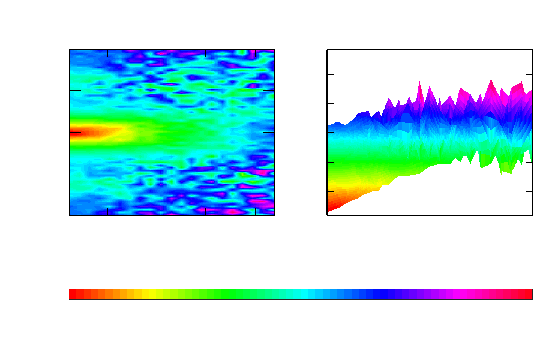
\includegraphics{./figures/face_bottom}}%
    \gplfronttext
  \end{picture}%
\endgroup
 \label{fig:b}}
  \caption{\small
           Given a 2D LIDAR sensor's measurement, at its core, CBGL disperses
           pose hypotheses within the map and ranks them ascendingly according
           to the value of the CAER metric, producing a \texttt{r}(ank)-field
           which may be used to estimate the pose of the sensor quickly due to
           the low complexity of the CAER metric.
           Top: a map of an environment, the pose of a panoramic 2D LIDAR sensor
           (magenta), and the corresponding CAER rank field below them.
           Bottom: distribution of CAER values by location and orientation
           error of all sensor pose hypotheses corresponding to the rank field
           above, for estimate distances up to $2.0$ m.
           In this example the map's area is $800$ m$^2$, and $10^6$ hypotheses
           were dispersed randomly in its free space for $100$ times; CBGL's
           maximum location error and maximum execution time were,
           respectively, $0.062$ m and $8.8$ sec
           }
  \vspace{-0.75cm}
  \label{fig:AB}
\end{figure}


%%%%%%%%%%%%%%%%%%%%%%%%%%%%%%%%%%%%%%%%%%%%%%%%%%%%%%%%%%%%%%%%%%%%%%%%%%%%%%%%
\section{Definitions and Problem Formulation}
  \label{section:definitions_and_problem_formulation}
  %%%%%%%%%%%%%%%%%%%%%%%%%%%%%%%%%%%%%%%%%%%%%%%%%%%%%%%%%%%%%%%%%%%%%%%%%%%%%%%%
\begin{definition}
  \label{def:definition_1}
  \textit{Definition of a range scan captured from a conventional 2D LIDAR
  sensor}. A conventional 2D LIDAR sensor provides a finite number of ranges,
  i.e. distances to objects within its range, on a horizontal cross-section of
  its environment, at regular angular and temporal intervals, over a defined
  angular range \cite{Cooper2018b}. A range scan $\mathcal{S}$, consisting
  of $N_s$ rays over an angular range $\lambda$, is an ordered map
  $\mathcal{S} : \Theta \rightarrow \mathbb{R}_{\geq 0}$, $\Theta =
  \{\theta_n \in [-\frac{\lambda}{2}, +\frac{\lambda}{2}) : \theta_n =
  -\frac{\lambda}{2} + \lambda \frac{n}{N_s}$, $n = 0,1,\dots, N_s$$-$$1$$\}$.
  Angles $\theta_n$ are expressed relative to the sensor's heading, in the
  sensor's frame of reference. The angular distance between two consecutive
  rays is the sensor's angle increment $\gamma \triangleq \lambda/N_s$.
\end{definition}

%%%%%%%%%%%%%%%%%%%%%%%%%%%%%%%%%%%%%%%%%%%%%%%%%%%%%%%%%%%%%%%%%%%%%%%%%%%%%%%%
\begin{definition}
  \label{def:definition_2}
  \textit{Definition of a map-scan}.
  A map-scan is a virtual scan that encapsulates the same pieces of information
  as a scan derived from a physical sensor. Only their underlying operating
  principle is different due to the fact the map-scan refers to distances to
  the boundaries of a point-set, referred to as the map, rather than within a
  real environment. A map-scan $\mathcal{S}_V^{\bm{M}}(\hat{\bm{p}})$ is
  derived by means of locating intersections of rays emanating from the
  estimate of the sensor's pose estimate $\hat{\bm{p}}$ and the boundaries of
  the map $\bm{M}$.
\end{definition}

%%%%%%%%%%%%%%%%%%%%%%%%%%%%%%%%%%%%%%%%%%%%%%%%%%%%%%%%%%%%%%%%%%%%%%%%%%%%%%%%
\begin{definition}
  \label{def:definition_3}
  \textit{The Cumulative Absolute Error per Ray (CAER) metric}.
  Let $\mathcal{S}_p$ and $\mathcal{S}_q$ be two range scans, equal in angular
  range $\lambda$ and size $N_s$. The value of the Cumulative Absolute Error
  per Ray metric $\psi \in \mathbb{R}_{\geq 0}$ between $\mathcal{S}_p$ and
  $\mathcal{S}_q$ is given by
  \begin{align}
    \psi(\mathcal{S}_p,\mathcal{S}_q) \triangleq \sum\limits_{n=0}^{N_s-1} \Big| \mathcal{S}_p[n]-\mathcal{S}_q[n]\Big| \nonumber
  \end{align}
\end{definition}

%%%%%%%%%%%%%%%%%%%%%%%%%%%%%%%%%%%%%%%%%%%%%%%%%%%%%%%%%%%%%%%%%%%%%%%%%%%%%%%%
\begin{customprb}{P}
  \label{prob:the_problem}
  Let the unknown pose of an immobile 2D range sensor whose angular range is
  $\lambda$ be $\bm{p}(x,y,\theta)$ with respect to the reference frame of map
  $\bm{M}$. Let the range sensor measure range scan $\mathcal{S}_R$. The
  objective is the estimation of $\bm{p}$ given $\bm{M}$, $\lambda$, and
  $\mathcal{S}_R$.
\end{customprb}

%%%%%%%%%%%%%%%%%%%%%%%%%%%%%%%%%%%%%%%%%%%%%%%%%%%%%%%%%%%%%%%%%%%%%%%%%%%%%%%%
\begin{customhpt}{H}
  \label{hpt:hypothesis_h1}
  Let the unknown pose of an 2D range sensor measuring range scan
  $\mathcal{S}_R$ be $\bm{p}(x,y,\theta)$ with respect to the reference frame
  of map $\bm{M}$.  Let $\mathcal{H}$ be a set of pose hypotheses within the
  free (i.e. traversable) space of $\bm{M}$:
  $\mathcal{H} = \{\hat{\bm{p}}_i\} \subseteq \texttt{free}(\bm{M})$, $i=0,1,\dots,|\mathcal{H}|-1$; $\mathbb{S}$
  be the set of map-scans (def. \ref{def:definition_2}) of $\bm{M}$ from pose
  hypotheses $\mathcal{H}$:
  $\mathbb{S} = \{\mathcal{S}_V^{\bm{M}}(\hat{\bm{p}}_i)\}$; and $\Psi$ be the
  set of CAERs (def. \ref{def:definition_3}) between $\mathcal{S}_R$ and the
  elements of $\mathbb{S}$:
  $\Psi = \{\psi(\mathcal{S}_R, \mathcal{S}_V^{\bm{M}}(\hat{\bm{p}}_i))\}$.
  Then there exist $\delta_0,\psi_0 \in \mathbb{R}_{> 0}$ which define a set of
  pose estimates $\mathcal{V} \subseteq \mathcal{H}$ such that
  \begin{align}
    \|\bm{p}-\hat{\bm{p}}_\mathcal{V}\|_2 &< \delta_0 \nonumber \text{ and}\\
    \psi(\mathcal{S}_R,\mathcal{S}_V^{\bm{M}}(\hat{\bm{p}}_\mathcal{V})) &< \psi_0 \nonumber
  \end{align}
  for all $\hat{\bm{p}}_\mathcal{V} \in \mathcal{V}$, for which
  \begin{align}
    \psi(\bm{p}, \hat{\bm{p}}_\mathcal{V}) &< \psi(\bm{p}, \hat{\bm{p}}_{\mathcal{H} \backslash \mathcal{V}}) \nonumber \\
    &\Rightarrow \nonumber \\
    \|\bm{p}-\hat{\bm{p}}_\mathcal{V}\|_2 &< \|\bm{p}-\hat{\bm{p}}_{\mathcal{H} \backslash \mathcal{V}}\|_2 \nonumber
  \end{align}
  for any $\hat{\bm{p}}_{\mathcal{H} \backslash \mathcal{V}} \in {\mathcal{H} \backslash \mathcal{V}}: \|\bm{p}-\hat{\bm{p}}_{\mathcal{H} \backslash \mathcal{V}}\|_2 \geq \delta_0$.

\end{customhpt}


%%%%%%%%%%%%%%%%%%%%%%%%%%%%%%%%%%%%%%%%%%%%%%%%%%%%%%%%%%%%%%%%%%%%%%%%%%%%%%%%
\section{Prior Work}
  \label{section:sota}
  The literature concerning the solution to the problem of global localisation
with the use of a 2D LIDAR sensor is rich; a brief overview is given below.

In broad terms global localisation approaches may be divided into two
categories: (a) approaches that operate in feature space, that is, methods that
extract features from measurements and the map and then establishing
correspondences between them, and (b) approaches that directly exploit only raw
measurements. In the latter category a number of global localisation methods
solve the problem in an iterative Bayesian Monte Carlo fashion, i.e. by
dispersing hypotheses within the map and updating the belief of the robot's
pose by incorporating new measurements as it moves until estimate convergence
\cite{mcl,Wang2018d,Yilmaz2019a,gmcl,Chen2021a}. However, the requirement of
motion (a) may give rise to safety concerns (the robot may not even be
visible), and (b) increases estimation time. The Monte Carlo method proposed in
this article operates directly in measurement space as well but, in contrast,
it does not require motion or more than one measurement. As a result CBGL is a
single-shot global localisation approach that is executable in less time
compared to previous Monte Carlo approaches.

Research on the former category has been more extensive due to the richness,
appropriateness, adaptability, and efficacy of methods originated in the
computer vision field. Relevant methods mainly perform detection of key-points
in a measurement, followed by the calculation of a distinctive signature,
which is then matched to similarly- and pre-computed place-signatures
\cite{Kallasi2016a,Usman2019,Wang2021b,Meng2021,Hendrikx2021,An2022,Nielsen2023}.
In principle, however, unstructured environments cannot be relied upon for the
existence of features, due to their complete absence or their sparse and
fortuitous distribution (although Deep Neural Network approaches have
demonstrated increased performance in place recognition with the use of 3D
LIDARs \cite{Xu2021,Yin2022,Komorowski2022}). Structured environments on the
other hand manifest different features depending on the particularities of the
environment. In any case, features may be present but not in a sufficiently
undisturbed state due to sensor noise or map-to-environment mismatch.

The motivation of the proposed method originates from seeking to achieve a
greater degree of universality, reliability, and portability across multiple
and disparate environments, by not making a priori assumptions on environment
structure, and by aiming to minimise requirements on resources (number and
types of sensors; number of measurements; time). The proposed method is most
akin to the two tested methods in \cite{Filotheou2022g}: all three are
single-shot 2D LIDAR-based Monte Carlo approaches, but CBGL computes a measure
of the alignment of (a) the measurement to (b) the virtual scan captured from
each hypothesis \textit{before} scan--to--map-scan matching a subset of the
most-aligned poses to the measurement. As a consequence it is able to process
more hypotheses in less time, resulting in (a) an improvement over the number
of correctly estimated locations and, most starkly, (b) execution time, being
able to compete against (traditionally faster) feature-based approaches.

A recent and comprehensive survey on global localisation may be found in
\cite{gl_survey_cn}.


%%%%%%%%%%%%%%%%%%%%%%%%%%%%%%%%%%%%%%%%%%%%%%%%%%%%%%%%%%%%%%%%%%%%%%%%%%%%%%%%
\section{Approach}
  \label{section:the_proposed_method}
  %%%%%%%%%%%%%%%%%%%%%%%%%%%%%%%%%%%%%%%%%%%%%%%%%%%%%%%%%%%%%%%%%%%%%%%%%%%%%%%%
%%%%%%%%%%%%%%%%%%%%%%%%%%%%%%%%%%%%%%%%%%%%%%%%%%%%%%%%%%%%%%%%%%%%%%%%%%%%%%%%
\subsection{Motivation}
\label{subsec:motivation}

The proposed method's motivation lies in the simple but powerful fact that in
general is exhibited through fig. \ref{fig:motivation_caer}: Let a pose
estimate of a 2D LIDAR sensor be in a neighbourhood of its true pose within a
given map (Def. \ref{def:definition_0}); then the value of the CAER metric
(Def.  \ref{def:definition_3}) between the scan measured by the sensor (Def.
\ref{def:definition_1}) and the map-scan captured from the estimate within the
map (Def. \ref{def:definition_2}) is proportional to both the estimate's
location error and orientation error. In other words comparing any two pose
estimates residing in a neighbourhood of the sensor's pose in terms of a scalar
value is enough to establish a pose error hierarchy between them. Moreover,
this scalar locus metric is directly derivable and calculable from the
assumptions of Problem \ref{prob:the_problem}, with low computational
complexity $\mathcal{O}(N_s)$.

The relationships of proportionality between the CAER metric of a pose
estimate and its location and orientation errors have been discovered and
successfully exploited in the context of non-global localisation, and
specifically in pose-tracking, for the production of lidar odometry
\cite{Filotheou2022f} and the reduction of localisation's pose estimate error
\cite{Filotheou2023a}. In this context, estimate errors are close to the
origin, i.e. in contrast to the arbitrary distribution of hypotheses' errors in
Monte Carlo global localisation methods.


\begin{figure}\vspace{-1.5cm}
  \subfloat{\hspace{0.5cm}% GNUPLOT: LaTeX picture with Postscript
\begingroup
  \makeatletter
  \providecommand\color[2][]{%
    \GenericError{(gnuplot) \space\space\space\@spaces}{%
      Package color not loaded in conjunction with
      terminal option `colourtext'%
    }{See the gnuplot documentation for explanation.%
    }{Either use 'blacktext' in gnuplot or load the package
      color.sty in LaTeX.}%
    \renewcommand\color[2][]{}%
  }%
  \providecommand\includegraphics[2][]{%
    \GenericError{(gnuplot) \space\space\space\@spaces}{%
      Package graphicx or graphics not loaded%
    }{See the gnuplot documentation for explanation.%
    }{The gnuplot epslatex terminal needs graphicx.sty or graphics.sty.}%
    \renewcommand\includegraphics[2][]{}%
  }%
  \providecommand\rotatebox[2]{#2}%
  \@ifundefined{ifGPcolor}{%
    \newif\ifGPcolor
    \GPcolorfalse
  }{}%
  \@ifundefined{ifGPblacktext}{%
    \newif\ifGPblacktext
    \GPblacktexttrue
  }{}%
  % define a \g@addto@macro without @ in the name:
  \let\gplgaddtomacro\g@addto@macro
  % define empty templates for all commands taking text:
  \gdef\gplfronttext{}%
  \gdef\gplfronttext{}%
  \makeatother
  \ifGPblacktext
    % no textcolor at all
    \def\colorrgb#1{}%
    \def\colorgray#1{}%
  \else
    % gray or color?
    \ifGPcolor
      \def\colorrgb#1{\color[rgb]{#1}}%
      \def\colorgray#1{\color[gray]{#1}}%
      \expandafter\def\csname LTw\endcsname{\color{white}}%
      \expandafter\def\csname LTb\endcsname{\color{black}}%
      \expandafter\def\csname LTa\endcsname{\color{black}}%
      \expandafter\def\csname LT0\endcsname{\color[rgb]{1,0,0}}%
      \expandafter\def\csname LT1\endcsname{\color[rgb]{0,1,0}}%
      \expandafter\def\csname LT2\endcsname{\color[rgb]{0,0,1}}%
      \expandafter\def\csname LT3\endcsname{\color[rgb]{1,0,1}}%
      \expandafter\def\csname LT4\endcsname{\color[rgb]{0,1,1}}%
      \expandafter\def\csname LT5\endcsname{\color[rgb]{1,1,0}}%
      \expandafter\def\csname LT6\endcsname{\color[rgb]{0,0,0}}%
      \expandafter\def\csname LT7\endcsname{\color[rgb]{1,0.3,0}}%
      \expandafter\def\csname LT8\endcsname{\color[rgb]{0.5,0.5,0.5}}%
    \else
      % gray
      \def\colorrgb#1{\color{black}}%
      \def\colorgray#1{\color[gray]{#1}}%
      \expandafter\def\csname LTw\endcsname{\color{white}}%
      \expandafter\def\csname LTb\endcsname{\color{black}}%
      \expandafter\def\csname LTa\endcsname{\color{black}}%
      \expandafter\def\csname LT0\endcsname{\color{black}}%
      \expandafter\def\csname LT1\endcsname{\color{black}}%
      \expandafter\def\csname LT2\endcsname{\color{black}}%
      \expandafter\def\csname LT3\endcsname{\color{black}}%
      \expandafter\def\csname LT4\endcsname{\color{black}}%
      \expandafter\def\csname LT5\endcsname{\color{black}}%
      \expandafter\def\csname LT6\endcsname{\color{black}}%
      \expandafter\def\csname LT7\endcsname{\color{black}}%
      \expandafter\def\csname LT8\endcsname{\color{black}}%
    \fi
  \fi
  \setlength{\unitlength}{0.0500bp}%
  \begin{picture}(6000.00,4000.00)%
    \gplgaddtomacro\gplfronttext{%
      \colorrgb{0.00,0.00,0.00}%
      \colorrgb{0.00,0.00,0.00}%
      \put(445,1460){\makebox(0,0)[r]{\strut{}\scriptsize $-\pi$}}%
      \colorrgb{0.00,0.00,0.00}%
      \put(822,1360){\makebox(0,0)[r]{\strut{}\scriptsize $-\pi/2$}}%
      \colorrgb{0.00,0.00,0.00}%
      \colorrgb{0.00,0.00,0.00}%
      \put(1199,1260){\makebox(0,0)[r]{\strut{}\scriptsize $0.0$}}%
      \colorrgb{0.00,0.00,0.00}%
      \colorrgb{0.00,0.00,0.00}%
      \put(1577,1160){\makebox(0,0)[r]{\strut{}\scriptsize $+\pi/2$}}%
      \colorrgb{0.00,0.00,0.00}%
      \put(1954,1060){\makebox(0,0)[r]{\strut{}\scriptsize $+\pi$}}%
      \colorrgb{0.00,0.00,0.00}%
      \colorrgb{0.00,0.00,0.00}%
      \put(2444,979){\makebox(0,0){\strut{}\scriptsize $0.0$}}%
      \colorrgb{0.00,0.00,0.00}%
      \put(3042,1057){\makebox(0,0){\strut{}\scriptsize $10.0$}}%
      \colorrgb{0.00,0.00,0.00}%
      \put(3642,1135){\makebox(0,0){\strut{}\scriptsize $20.0$}}%
      \colorrgb{0.00,0.00,0.00}%
      \put(4241,1213){\makebox(0,0){\strut{}\scriptsize $30.0$}}%
      \colorrgb{0.00,0.00,0.00}%
      \put(594,1526){\makebox(0,0)[r]{\strut{}\scriptsize $0$}}%
      \colorrgb{0.00,0.00,0.00}%
      \put(594,1869){\makebox(0,0)[r]{\strut{}\scriptsize $400$}}%
      \colorrgb{0.00,0.00,0.00}%
      \put(594,2212){\makebox(0,0)[r]{\strut{}\scriptsize $800$}}%
      \colorrgb{0.00,0.00,0.00}%
      \put(594,2555){\makebox(0,0)[r]{\strut{}\scriptsize $1200$}}%
      \colorrgb{0.00,0.00,0.00}%
      %\put(-115,2129){\rotatebox{90}{\makebox(0,0){\strut{}\scriptsize CAER [m]}}}%
      \colorrgb{0.00,0.00,0.00}%
      %\put(2640,2854){\makebox(0,0){\strut{}title}}%
    }%
    \gplgaddtomacro\gplfronttext{%
      \colorrgb{0.00,0.00,0.00}%
      \put(679,1037){\rotatebox{-22}{\makebox(0,0){\strut{}\footnotesize Orientation error $\Delta\hat{\theta}$ [rad]}}}%
      \colorrgb{0.00,0.00,0.00}%
      \put(3621,852){\rotatebox{7}{\makebox(0,0){\strut{}\footnotesize Position error $\|\Delta\hat{\bm{l}}\|_2$ [m]}}}%
      \colorrgb{0.00,0.00,0.00}%
      \put(-115,2129){\rotatebox{90}{\makebox(0,0){\strut{}\footnotesize CAER [m]}}}%
    }%
    \gplgaddtomacro\gplfronttext{%
    }%
    \gplgaddtomacro\gplfronttext{%
      \colorrgb{0.00,0.00,0.00}%
%      \put(5375,1039){\makebox(0,0)[l]{\strut{}\scriptsize $0$}}%
      %\colorrgb{0.00,0.00,0.00}%
      %\put(5375,1624){\makebox(0,0)[l]{\strut{}\scriptsize $400$}}%
      %\colorrgb{0.00,0.00,0.00}%
      %\put(5375,2209){\makebox(0,0)[l]{\strut{}\scriptsize $800$}}%
      %\colorrgb{0.00,0.00,0.00}%
      %\put(5375,2795){\makebox(0,0)[l]{\strut{}\scriptsize $1200$}}%
      %\colorrgb{0.00,0.00,0.00}%
      %\put(5375,3087){\makebox(0,0)[l]{\strut{}\scriptsize $1400$}}%
    }%
    \put(0,0){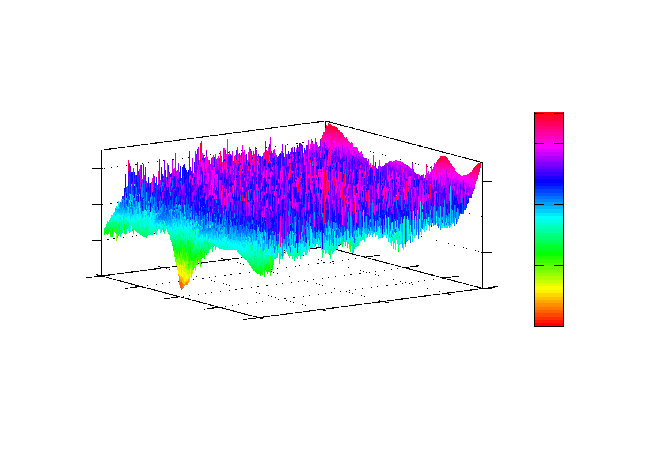
\includegraphics[trim={0 0 2cm 1.4cm},clip]{./figures/caer_all}}%
    \gplfronttext
  \end{picture}%
\endgroup
}\vspace{-1.5cm}\\
  \subfloat{\hspace{-0.3cm}% GNUPLOT: LaTeX picture with Postscript
\begingroup
  \makeatletter
  \providecommand\color[2][]{%
    \GenericError{(gnuplot) \space\space\space\@spaces}{%
      Package color not loaded in conjunction with
      terminal option `colourtext'%
    }{See the gnuplot documentation for explanation.%
    }{Either use 'blacktext' in gnuplot or load the package
      color.sty in LaTeX.}%
    \renewcommand\color[2][]{}%
  }%
  \providecommand\includegraphics[2][]{%
    \GenericError{(gnuplot) \space\space\space\@spaces}{%
      Package graphicx or graphics not loaded%
    }{See the gnuplot documentation for explanation.%
    }{The gnuplot epslatex terminal needs graphicx.sty or graphics.sty.}%
    \renewcommand\includegraphics[2][]{}%
  }%
  \providecommand\rotatebox[2]{#2}%
  \@ifundefined{ifGPcolor}{%
    \newif\ifGPcolor
    \GPcolorfalse
  }{}%
  \@ifundefined{ifGPblacktext}{%
    \newif\ifGPblacktext
    \GPblacktexttrue
  }{}%
  % define a \g@addto@macro without @ in the name:
  \let\gplgaddtomacro\g@addto@macro
  % define empty templates for all commands taking text:
  \gdef\gplfronttext{}%
  \gdef\gplfronttext{}%
  \makeatother
  \ifGPblacktext
    % no textcolor at all
    \def\colorrgb#1{}%
    \def\colorgray#1{}%
  \else
    % gray or color?
    \ifGPcolor
      \def\colorrgb#1{\color[rgb]{#1}}%
      \def\colorgray#1{\color[gray]{#1}}%
      \expandafter\def\csname LTw\endcsname{\color{white}}%
      \expandafter\def\csname LTb\endcsname{\color{black}}%
      \expandafter\def\csname LTa\endcsname{\color{black}}%
      \expandafter\def\csname LT0\endcsname{\color[rgb]{1,0,0}}%
      \expandafter\def\csname LT1\endcsname{\color[rgb]{0,1,0}}%
      \expandafter\def\csname LT2\endcsname{\color[rgb]{0,0,1}}%
      \expandafter\def\csname LT3\endcsname{\color[rgb]{1,0,1}}%
      \expandafter\def\csname LT4\endcsname{\color[rgb]{0,1,1}}%
      \expandafter\def\csname LT5\endcsname{\color[rgb]{1,1,0}}%
      \expandafter\def\csname LT6\endcsname{\color[rgb]{0,0,0}}%
      \expandafter\def\csname LT7\endcsname{\color[rgb]{1,0.3,0}}%
      \expandafter\def\csname LT8\endcsname{\color[rgb]{0.5,0.5,0.5}}%
    \else
      % gray
      \def\colorrgb#1{\color{black}}%
      \def\colorgray#1{\color[gray]{#1}}%
      \expandafter\def\csname LTw\endcsname{\color{white}}%
      \expandafter\def\csname LTb\endcsname{\color{black}}%
      \expandafter\def\csname LTa\endcsname{\color{black}}%
      \expandafter\def\csname LT0\endcsname{\color{black}}%
      \expandafter\def\csname LT1\endcsname{\color{black}}%
      \expandafter\def\csname LT2\endcsname{\color{black}}%
      \expandafter\def\csname LT3\endcsname{\color{black}}%
      \expandafter\def\csname LT4\endcsname{\color{black}}%
      \expandafter\def\csname LT5\endcsname{\color{black}}%
      \expandafter\def\csname LT6\endcsname{\color{black}}%
      \expandafter\def\csname LT7\endcsname{\color{black}}%
      \expandafter\def\csname LT8\endcsname{\color{black}}%
    \fi
  \fi
    \setlength{\unitlength}{0.0500bp}%
    \ifx\gptboxheight\undefined%
      \newlength{\gptboxheight}%
      \newlength{\gptboxwidth}%
      \newsavebox{\gptboxtext}%
    \fi%
    \setlength{\fboxrule}{0.5pt}%
    \setlength{\fboxsep}{1pt}%
\begin{picture}(5000.00,3000.00)%
    \gplgaddtomacro\gplfronttext{%
    }%
    \gplgaddtomacro\gplfronttext{%
      \colorrgb{0.15,0.15,0.15}%
      \put(336,1498){\makebox(0,0)[r]{\strut{}}}%
      \colorrgb{0.15,0.15,0.15}%
      \put(336,1905){\makebox(0,0)[r]{\strut{}}}%
      \colorrgb{0.15,0.15,0.15}%
      \put(336,2312){\makebox(0,0)[r]{\strut{}}}%
      \colorrgb{0.15,0.15,0.15}%
      \put(300,1905){\rotatebox{90}{\makebox(0,0){\strut{}$\Delta\hat{\theta} \in [-\pi,\pi)$ rad}}}%
      %\put(400,933){\makebox(0,0){\strut{}\small $0.0$}}%
      \colorrgb{0.15,0.15,0.15}%
      \put(871,933){\makebox(0,0){\strut{}\small $0.5$}}%
      \colorrgb{0.15,0.15,0.15}%
      \put(1342,933){\makebox(0,0){\strut{}\small $1.0$}}%
      \colorrgb{0.15,0.15,0.15}%
      \put(1813,933){\makebox(0,0){\strut{}\small $1.5$}}%
      \colorrgb{0.15,0.15,0.15}%
      \put(2285,933){\makebox(0,0){\strut{}\small $2.0$}}%
      \colorrgb{0.15,0.15,0.15}%
      \put(1487,663){\makebox(0,0){\strut{}$\|\Delta \hat{\bm{l}}\|_2$ [m]}}%
    }%
    \gplgaddtomacro\gplfronttext{%
    }%
    \gplgaddtomacro\gplfronttext{%
      \colorrgb{0.15,0.15,0.15}%
      \put(5113,1110){\makebox(0,0)[l]{\strut{}}}%
      \colorrgb{0.15,0.15,0.15}%
      \put(5113,1110){\makebox(0,0)[l]{\strut{}}}%
      \colorrgb{0.15,0.15,0.15}%
      \put(5113,1110){\makebox(0,0)[l]{\strut{}}}%
      %\put(2875,933){\makebox(0,0){\strut{}\small $0.0$}}%
      \colorrgb{0.15,0.15,0.15}%
      \put(3346,933){\makebox(0,0){\strut{}\small $0.5$}}%
      \colorrgb{0.15,0.15,0.15}%
      \put(3817,933){\makebox(0,0){\strut{}\small $1.0$}}%
      \colorrgb{0.15,0.15,0.15}%
      \put(4288,933){\makebox(0,0){\strut{}\small $1.5$}}%
      \colorrgb{0.15,0.15,0.15}%
      \put(4760,933){\makebox(0,0){\strut{}\small $2.0$}}%
      \colorrgb{0.15,0.15,0.15}%
      \put(2762,1905){\rotatebox{90}{\makebox(0,0){\strut{}\small CAER [m]}}}
      \put(3987,663){\makebox(0,0){\strut{}$\|\Delta \hat{\bm{l}}\|_2$ [m]}}%
    }%
    \gplgaddtomacro\gplfronttext{%
    }%
    \gplgaddtomacro\gplfronttext{%
    }%
    \gplgaddtomacro\gplfronttext{%
    }%
    \gplgaddtomacro\gplfronttext{%
      \put(500,80){\makebox(0,0){\strut{}$\footnotesize 0$}}%
      \colorrgb{0.15,0.15,0.15}%
%      \put(1390,80){\makebox(0,0){\strut{}$\footnotesize 60$}}%
      %\colorrgb{0.15,0.15,0.15}%
      %\put(2280,80){\makebox(0,0){\strut{}$\footnotesize 270$}}%
      %\colorrgb{0.15,0.15,0.15}%
      %\put(3169,80){\makebox(0,0){\strut{}$\footnotesize 540$}}%
      %\colorrgb{0.15,0.15,0.15}%
      %\put(4059,80){\makebox(0,0){\strut{}$\footnotesize 810$}}%
      \colorrgb{0.15,0.15,0.15}%
      \put(4849,80){\makebox(0,0){\strut{}$\footnotesize 1080$}}%
    }%
    \put(0,0){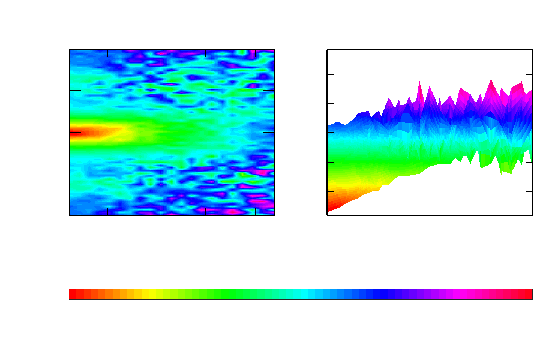
\includegraphics{./figures/face_bottom}}%
    \gplfronttext
  \end{picture}%
\endgroup
}
  \caption{\small Top: without loss o generality, a typical plot of the
           Cumulative Absolute Error per Ray metric (Eq. (\ref{eq:caer})) of
           $10^6$ hypotheses disperesed in the map of environment WAREHOUSE
           (Fig. \ref{fig:face} and section \ref{subsec:exp_b}). Bottom:
           focused view on hypotheses with location error close to the origin}
  \vspace{-0.5cm}
  \label{fig:motivation_caer}
\end{figure}


The above motivate investigation on whether the CAER metric could prove equally
beneficial in settings more uncertain than pose-tracking, that is, where the
location and orientation of pose estimates extend farther away from the
sensor's true location and orientation. Fig. \ref{fig:h_and_h_not_fig} (top)
shows the relations between the total errors of hypotheses and
their (a) CAER values (left) and (b) resulting ranks (right),
which resulted from an experimental procedure similar to that which produced fig.
\ref{fig:motivation_caer}.

%%%%%%%%%%%%%%%%%%%%%%%%%%%%%%%%%%%%%%%%%%%%%%%%%%%%%%%%%%%%%%%%%%%%%%%%%%%%%%%%
%%%%%%%%%%%%%%%%%%%%%%%%%%%%%%%%%%%%%%%%%%%%%%%%%%%%%%%%%%%%%%%%%%%%%%%%%%%%%%%%
\subsection{The CBGL System}

In order to test the efficacy of the CAER metric in aiding the solution of
Problem \ref{prob:the_problem}, we introduce the CAER-Based Global Localisation
system (CBGL).\footnote{For a rigorous mathematical formulation of the
hypothesis underpinning CBGL see \cite{cbglarxiv}.} Given map $\bm{M}$, CBGL
first generates a set of pose hypotheses $\mathcal{H}$ (Def.
\ref{def:definition_0}). Their positions are randomly generated
uniformly within the map's traversable space, while orientations within
$[-\pi,\pi)$ rad. Then from these poses it computes map-scans (Def.
\ref{def:definition_2}). Given these map-scans and a LIDAR's 2D measurement
$\mathcal{S}_R$ (Def. \ref{def:definition_1}), CBGL subsequently computes the
CAER value (Def. \ref{def:definition_3}) associated with each pose hypothesis.
It then ranks them in ascending order and selects the $k$ estimates with the
least CAER values in an attempt to estimate the $k$ hypotheses with the least
pose error (Alg. \ref{alg:bottom_k}). Estimation in this sense rests on the
motivation of subsection \ref{subsec:motivation}.

One challenge is choosing such $k$, $d_{\bm{l}}$, and $d_\alpha$ (Def.
\ref{def:definition_6}) that, given pose estimate error requirements
$\delta_{\bm{l}}$, $\delta_{\theta}$, CBGL produces admissible pose estimates
(Def. \ref{def:definition_7}) while being executed in timely manner.  Given the
rank field's Monte Carlo nature, optimistically, the only option for increasing
the accuracy of the final pose estimate by a factor of two would be to double
the densities of the \texttt{r}-field; instead of doing that---and thereby
doubling the method's execution time---subsequent to the estimation of the pose
estimates with the $k$ lowest CAER values, CBGL utilises scan--to--map-scan
matching \cite{Vasiljevic2016c,Filotheou2023a}, followed by the estimation of
the one pose estimate with the lowest CAER value within the group of $k$
matched estimates.

Matching allows for (a) the correction of the pose of true positive estimates
by scan-matching the map-scan captured from a pose estimate against the range
scan measured by the real sensor, (b) by the same token the potential
divergence of spurious, false positive, pose estimates, and hence their
elimination as pose estimate candidates, (c) the production of finer pose
estimates without excessive increase in execution time, and (d) the decoupling
of the final pose estimate's error from the field's densities.

CBGL's output pose estimate is that with the least CAER among the $k$ matched
estimates. CBGL is described in block diagram form in figure
\ref{fig:block_system} (left) and in pseudocode in Algorithm \ref{alg:cbgl}.


\begin{figure}\vspace{-0.4cm}
  \subfloat{\label{fig:cbgl}     \input{./figures/cbgl_system_tiny.tikz}}
  \subfloat{\label{fig:bottom_k} \input{./figures/inner_ranking_system2_tiny.tikz}}
  \caption{\small CBGL in block diagram form. Left: Given map $\bm{M}$, CBGL
           first generates a set of pose hypotheses $\mathcal{H}$. Then it
           estimates the $k$ hypotheses with the least pose error (right; Alg.
           \ref{alg:bottom_k}).
           %II \cite{Filotheou2023c}
           As a final step, it scan--to--map-scan
           matches these to $\mathcal{S}_R$ for finer estimation
           (\texttt{sm2}; Alg.
           \ref{alg:sm2}).
           %III \cite{Filotheou2023c}
           CBGL's output pose estimate is that with
           the minimum CAER among the $k$ matched estimates
           }
\vspace{-0.5cm}
  \label{fig:block_system}
\end{figure}


%%% CBGL %%%%%%%%%%%%%%%%%%%%%%%%%%%%%%%%%%%%%%%%%%%%%%%%%%%%%%%%%%%%%%%%%%%%%%%%
\begin{algorithm}[]
  \caption{\texttt{CBGL}}
  \begin{spacing}{1.0}
  \begin{algorithmic}[1]
    \REQUIRE $\mathcal{S}_R$, $\lambda$, $\bm{M}$, $(d_{\bm{l}}, d_\alpha)$, $k$
    \ENSURE Pose estimate of sensor measuring range scan $\mathcal{S}_R$ %$\hat{\bm{p}}$
    \STATE $A \leftarrow \texttt{calculate\_area}(\texttt{free}(\bm{M}))$
    \STATE $\mathcal{H} \leftarrow \{\varnothing\}$
    \FOR {$i \leftarrow 0,1,\dots,d_{\bm{l}} \cdot A-1$}
      \STATE \small $(\hat{x},\hat{y},\hat{\theta}) \leftarrow \texttt{rand()}$: $(x,y) \in \texttt{free}(\bm{M})$, $\hat{\theta} \in [-\pi,+\pi)$
      \FOR {$j \leftarrow 0,1,\dots, d_{\alpha}-1$}
        \STATE $\mathcal{H} \leftarrow \{\mathcal{H}, (\hat{x}, \hat{y}, \hat{\theta} + j \cdot 2\pi / d_{\alpha})\}$     \label{alg:cbgl:h}
      \ENDFOR
    \ENDFOR
    \STATE $\mathcal{H}_1 \leftarrow$ \texttt{bottom}$\_k\_\texttt{poses}(\mathcal{S}_R, \bm{M}, \mathcal{H}, k)$ \hfill {\small (Alg. \ref{alg:bottom_k}}) \label{alg:cbgl:h1}
    \STATE $\mathcal{H}_2 \leftarrow \{\varnothing \}$
    \FOR {$k \leftarrow 0,1,\dots,|\mathcal{H}_1|-1$}
      \STATE $\hat{\bm{h}}^\prime \leftarrow \texttt{sm2}(\mathcal{S}_R, \lambda, \bm{M}, \mathcal{H}_1[k])$ \hfill {\small (Alg. \ref{alg:sm2}---e.g. \texttt{x1} \cite{Filotheou2023a}})
      \STATE $\mathcal{H}_2 \leftarrow \{\mathcal{H}_2, \hat{\bm{h}}^\prime\}$  \label{alg:cbgl:h2}
    \ENDFOR
    \RETURN \texttt{bottom}$\_k\_\texttt{poses}(\mathcal{S}_R, \bm{M}, \mathcal{H}_2, 1)$
  \end{algorithmic}
  \end{spacing}
  \label{alg:cbgl}
\end{algorithm}

%% Bottom-n %%%%%%%%%%%%%%%%%%%%%%%%%%%%%%%%%%%%%%%%%%%%%%%%%%%%%%%%%%%%%%%%%%%%
\begin{algorithm}[]
  \caption{\texttt{bottom}\_$k$\_\texttt{poses}}
  \begin{spacing}{1.0}
  \begin{algorithmic}[1]
    \REQUIRE $\mathcal{S}_R$, $\bm{M}$, $\mathcal{H}$, $k$
    \ENSURE Set of $k$ poses of $\mathcal{H}$ with least CAER values, $\mathcal{H}_{\triangledown}$
    \STATE $\Psi \leftarrow \{\varnothing \}$
    \FOR {$h \leftarrow 0,1,\dots,|\mathcal{H}|-1$}
      \STATE $\mathcal{S}_V^{\hspace{1pt} h} \leftarrow \texttt{scan\_map}(\bm{M}, \mathcal{H}[h])$
      \STATE $\psi \leftarrow 0$
      \FOR {$n \leftarrow 0,1,\dots,|\mathcal{S}_R|-1$}
        \STATE $\psi \leftarrow \psi + \big|\mathcal{S}_R[n]-\mathcal{S}_V^{\hspace{1pt} h}[n]\big|$ \hfill {\small (Eq. (\ref{eq:caer})})
      \ENDFOR
      \STATE $\Psi \leftarrow \{\Psi, \psi\}$
    \ENDFOR
    \STATE $[\Psi_{\uparrow}, \texttt{I}^{\ast}] \leftarrow \texttt{sort}(\Psi, \texttt{asc})$
    \STATE $\mathcal{H}_{\triangledown} \leftarrow \{\varnothing \}$
    \FOR {$h \leftarrow 0,1,\dots,k-1$}
      \STATE $\mathcal{H}_{\triangledown} \leftarrow \{\mathcal{H}_{\triangledown}, \mathcal{H}[\texttt{I}^{\ast}[h]]\}$
    \ENDFOR
    \RETURN $\mathcal{H}_{\triangledown}$
  \end{algorithmic}
  \end{spacing}
  \label{alg:bottom_k}
\end{algorithm}

%% sm2 %%%%%%%%%%%%%%%%%%%%%%%%%%%%%%%%%%%%%%%%%%%%%%%%%%%%%%%%%%%%%%%%%%%%%%%%%
\begin{algorithm}[]
  \caption{\texttt{sm2}}
  \begin{spacing}{1.0}
  \begin{algorithmic}[1]
    \REQUIRE $\mathcal{S}_R$, $\lambda$, $\bm{M}$, $\hat{\bm{p}}$
    %\ENSURE $\hat{\bm{p}}^\prime$
    \ENSURE $\hat{\bm{p}}$ $+$ correction that aligns $\mathcal{S}_V^{\bm{M}}(\hat{\bm{p}})$ to $\mathcal{S}_R$
    \STATE $\mathcal{S}_V \leftarrow \texttt{scan\_map}(\bm{M}, \hat{\bm{p}}, \lambda)$
    \STATE $\bm{\Delta p} \leftarrow \texttt{scan-match}(\mathcal{S}_R,\mathcal{S}_V)$ \hfill {\small (e.g. \texttt{ICP}\cite{Vizzo2023}, \texttt{FSM}\cite{Filotheou2022f}})
    %\STATE $\hat{\bm{p}}^\prime \leftarrow \hat{\bm{p}} + \bm{\Delta p}$
    %\RETURN $\hat{\bm{p}}^\prime$
    \RETURN $\hat{\bm{p}} + \bm{\Delta p}$
  \end{algorithmic}
  \end{spacing}
  \label{alg:sm2}
\end{algorithm}


%%%%%%%%%%%%%%%%%%%%%%%%%%%%%%%%%%%%%%%%%%%%%%%%%%%%%%%%%%%%%%%%%%%%%%%%%%%%%%%%
\section{Results}
  \label{section:results}
  This section serves the testing of Hypothesis \ref{hpt:hypothesis_h} under
state of the global localisation art methods and CBGL, in varying environmental
conditions and sensor configurations. With regard to CBGL its three required
parameters were set to $(d_{\bm{l}},d_{\alpha},k) = (40, 2^5, 10)$ after
preparatory tests with the dataset tested against in subsection
\ref{subsec:exp_in_re_co}. The rationale of choosing appropriate
$d_{\bm{l}},d_{\alpha}$ is depicted in figure \ref{fig:a:determine_40_32}, and
$k$ was chosen as such in order to retain a high-enough true positive discovery
rate without significant increase in execution time (due to the application of
scan--to--map-scan matching on $k$ pose estimates).


\subsection{Experiments in real conditions}
\label{subsec:exp_in_re_co}

The first type of tests were conducted with the use of a Hokuyo UTM-30LX
sensor, whose angular range is $\lambda = 3\pi/2$ rad and maximum range
$r_{\max} = 30.0$ m, in the  Electrical and Computer Engineering Department's
Laboratory of Computer Systems Architecture (CSAL), Aristotle University of
Thessaloniki, Greece, a map of which is depicted in figure
\ref{fig:a:map_and_trajectory}. The sensor was mounted on a Robotnik RB1 robot,
which was teleoperated to move within the environment while range scans were
being captured. This resulted in $N_{S}=6669$ range scans, whose number of rays
were downsampled by a factor of four before being inputted to CBGL and ALS
\cite{als_jp}, an algorithm which implements Free-Space Features
\cite{als_eth}. CBGL's internal scan--to--map-scan matching method was chosen
to be PLICP \cite{Censi2008c} due to its low execution time and the scans'
non-panoramic field of view.  Other global localisation methods ?? were not to
tested for this type of experiment due to their infeasible execution time with
respect to the range dataset's volume. The top of figure \ref{fig:a:awesomeness}
depicts the proportion of output pose estimates from each method whose position
and orientation error was lower than varying values of outlier thresholds
$\delta_{\bm{l}}$, $\delta_{\theta}$; at the bottom they are depicted
exclusively with regard to CBGL's output and its internal pose sets. The mean
and standard deviation of the two methods' execution times were
$(\overline{\mu}_t^{\text{ALS}}, \sigma_t^{\text{ALS}}) = (6.15, 5.32)$ sec,
and $(\overline{\mu}_t^{\text{CBGL}}, \sigma_t^{\text{CBGL}}) = (1.61, 0.06)$
sec. From the experimental evidence it is clear that (a) hypothesis
\ref{hpt:hypothesis_h} is observed to be true $991$ times out of a thousand for
an outliers' locational threshold $\delta_{\bm{l}} = 0.5$ m when an angular
threshold is $\delta_{\theta}$ is not enforced, and (b) CBGL outperforms ALS in
terms of number of pose estimates within all locational and angular thresholds
and in terms of execution time.

\begin{figure}
  % GNUPLOT: LaTeX picture with Postscript
\begingroup
  \makeatletter
  \providecommand\color[2][]{%
    \GenericError{(gnuplot) \space\space\space\@spaces}{%
      Package color not loaded in conjunction with
      terminal option `colourtext'%
    }{See the gnuplot documentation for explanation.%
    }{Either use 'blacktext' in gnuplot or load the package
      color.sty in LaTeX.}%
    \renewcommand\color[2][]{}%
  }%
  \providecommand\includegraphics[2][]{%
    \GenericError{(gnuplot) \space\space\space\@spaces}{%
      Package graphicx or graphics not loaded%
    }{See the gnuplot documentation for explanation.%
    }{The gnuplot epslatex terminal needs graphicx.sty or graphics.sty.}%
    \renewcommand\includegraphics[2][]{}%
  }%
  \providecommand\rotatebox[2]{#2}%
  \@ifundefined{ifGPcolor}{%
    \newif\ifGPcolor
    \GPcolorfalse
  }{}%
  \@ifundefined{ifGPblacktext}{%
    \newif\ifGPblacktext
    \GPblacktexttrue
  }{}%
  % define a \g@addto@macro without @ in the name:
  \let\gplgaddtomacro\g@addto@macro
  % define empty templates for all commands taking text:
  \gdef\gplfronttext{}%
  \gdef\gplfronttext{}%
  \makeatother
  \ifGPblacktext
    % no textcolor at all
    \def\colorrgb#1{}%
    \def\colorgray#1{}%
  \else
    % gray or color?
    \ifGPcolor
      \def\colorrgb#1{\color[rgb]{#1}}%
      \def\colorgray#1{\color[gray]{#1}}%
      \expandafter\def\csname LTw\endcsname{\color{white}}%
      \expandafter\def\csname LTb\endcsname{\color{black}}%
      \expandafter\def\csname LTa\endcsname{\color{black}}%
      \expandafter\def\csname LT0\endcsname{\color[rgb]{1,0,0}}%
      \expandafter\def\csname LT1\endcsname{\color[rgb]{0,1,0}}%
      \expandafter\def\csname LT2\endcsname{\color[rgb]{0,0,1}}%
      \expandafter\def\csname LT3\endcsname{\color[rgb]{1,0,1}}%
      \expandafter\def\csname LT4\endcsname{\color[rgb]{0,1,1}}%
      \expandafter\def\csname LT5\endcsname{\color[rgb]{1,1,0}}%
      \expandafter\def\csname LT6\endcsname{\color[rgb]{0,0,0}}%
      \expandafter\def\csname LT7\endcsname{\color[rgb]{1,0.3,0}}%
      \expandafter\def\csname LT8\endcsname{\color[rgb]{0.5,0.5,0.5}}%
    \else
      % gray
      \def\colorrgb#1{\color{black}}%
      \def\colorgray#1{\color[gray]{#1}}%
      \expandafter\def\csname LTw\endcsname{\color{white}}%
      \expandafter\def\csname LTb\endcsname{\color{black}}%
      \expandafter\def\csname LTa\endcsname{\color{black}}%
      \expandafter\def\csname LT0\endcsname{\color{black}}%
      \expandafter\def\csname LT1\endcsname{\color{black}}%
      \expandafter\def\csname LT2\endcsname{\color{black}}%
      \expandafter\def\csname LT3\endcsname{\color{black}}%
      \expandafter\def\csname LT4\endcsname{\color{black}}%
      \expandafter\def\csname LT5\endcsname{\color{black}}%
      \expandafter\def\csname LT6\endcsname{\color{black}}%
      \expandafter\def\csname LT7\endcsname{\color{black}}%
      \expandafter\def\csname LT8\endcsname{\color{black}}%
    \fi
  \fi
    \setlength{\unitlength}{0.0500bp}%
    \ifx\gptboxheight\undefined%
      \newlength{\gptboxheight}%
      \newlength{\gptboxwidth}%
      \newsavebox{\gptboxtext}%
    \fi%
    \setlength{\fboxrule}{0.5pt}%
    \setlength{\fboxsep}{1pt}%
\begin{picture}(4500.00,4000.00)%
    \gplgaddtomacro\gplfronttext{%
      \colorrgb{0.15,0.15,0.15}%
      \put(318,2666){\makebox(0,0)[r]{\strut{}\footnotesize $0$}}%
      \colorrgb{0.15,0.15,0.15}%
      \put(318,2899){\makebox(0,0)[r]{\strut{}\footnotesize $500$}}%
      \colorrgb{0.15,0.15,0.15}%
      \put(318,3133){\makebox(0,0)[r]{\strut{}\footnotesize $1000$}}%
      \colorrgb{0.15,0.15,0.15}%
      \put(318,3366){\makebox(0,0)[r]{\strut{}\footnotesize $1500$}}%
      \colorrgb{0.15,0.15,0.15}%
      \put(318,3599){\makebox(0,0)[r]{\strut{}\footnotesize $2000$}}%
      \colorrgb{0.15,0.15,0.15}%
      \put(498,2566){\makebox(0,0){\strut{}\scriptsize $0$}}%
      \colorrgb{0.15,0.15,0.15}%
      \put(688,2566){\makebox(0,0){\strut{}\scriptsize $2$}}%
      \colorrgb{0.15,0.15,0.15}%
      \put(879,2566){\makebox(0,0){\strut{}\scriptsize $4$}}%
      \colorrgb{0.15,0.15,0.15}%
      \put(1070,2566){\makebox(0,0){\strut{}\scriptsize $6$}}%
      \colorrgb{0.15,0.15,0.15}%
      \put(1261,2566){\makebox(0,0){\strut{}\scriptsize $8$}}%
      \colorrgb{0.15,0.15,0.15}%
      \put(1451,2566){\makebox(0,0){\strut{}\scriptsize $10$}}%
    }%
    \gplgaddtomacro\gplfronttext{%
      \colorrgb{0.15,0.15,0.15}%
      \put(974,3716){\makebox(0,0){\strut{}\footnotesize $d_{\alpha} = 2^3$}}%
    }%
    \gplgaddtomacro\gplfronttext{%
      \colorrgb{0.15,0.15,0.15}%
      \put(1592,2666){\makebox(0,0)[r]{\strut{}}}%
      \colorrgb{0.15,0.15,0.15}%
      \put(1592,2899){\makebox(0,0)[r]{\strut{}}}%
      \colorrgb{0.15,0.15,0.15}%
      \put(1592,3133){\makebox(0,0)[r]{\strut{}}}%
      \colorrgb{0.15,0.15,0.15}%
      \put(1592,3366){\makebox(0,0)[r]{\strut{}}}%
      \colorrgb{0.15,0.15,0.15}%
      \put(1592,3599){\makebox(0,0)[r]{\strut{}}}%
      \colorrgb{0.15,0.15,0.15}%
      \put(1772,2566){\makebox(0,0){\strut{}\scriptsize $0$}}%
      \colorrgb{0.15,0.15,0.15}%
      \put(1963,2566){\makebox(0,0){\strut{}\scriptsize $2$}}%
      \colorrgb{0.15,0.15,0.15}%
      \put(2154,2566){\makebox(0,0){\strut{}\scriptsize $4$}}%
      \colorrgb{0.15,0.15,0.15}%
      \put(2356,2566){\makebox(0,0){\strut{}\scriptsize $6$}}%
      \colorrgb{0.15,0.15,0.15}%
      \put(2535,2566){\makebox(0,0){\strut{}\scriptsize $8$}}%
      \colorrgb{0.15,0.15,0.15}%
      \put(2726,2566){\makebox(0,0){\strut{}\scriptsize $10$}}%
    }%
    \gplgaddtomacro\gplfronttext{%
      \colorrgb{0.15,0.15,0.15}%
      \put(2249,3716){\makebox(0,0){\strut{}\footnotesize $d_{\alpha} = 2^4$}}%
    }%
    \gplgaddtomacro\gplfronttext{%
      \colorrgb{0.15,0.15,0.15}%
      \put(3048,2566){\makebox(0,0){\strut{}\scriptsize $0$}}%
      \colorrgb{0.15,0.15,0.15}%
      \put(3238,2566){\makebox(0,0){\strut{}\scriptsize $2$}}%
      \colorrgb{0.15,0.15,0.15}%
      \put(3429,2566){\makebox(0,0){\strut{}\scriptsize $4$}}%
      \colorrgb{0.15,0.15,0.15}%
      \put(3620,2566){\makebox(0,0){\strut{}\scriptsize $6$}}%
      \colorrgb{0.15,0.15,0.15}%
      \put(3811,2566){\makebox(0,0){\strut{}\scriptsize $8$}}%
      \colorrgb{0.15,0.15,0.15}%
      \put(4001,2566){\makebox(0,0){\strut{}\scriptsize $10$}}%
      \colorrgb{0.15,0.15,0.15}%
      \put(4181,2666){\makebox(0,0)[l]{\strut{}\footnotesize $0$}}%
      \colorrgb{0.15,0.15,0.15}%
      \put(4181,2899){\makebox(0,0)[l]{\strut{}\footnotesize $500$}}%
      \colorrgb{0.15,0.15,0.15}%
      \put(4181,3133){\makebox(0,0)[l]{\strut{}\footnotesize $1000$}}%
      \colorrgb{0.15,0.15,0.15}%
      \put(4181,3366){\makebox(0,0)[l]{\strut{}\footnotesize $1500$}}%
      \colorrgb{0.15,0.15,0.15}%
      \put(4181,3599){\makebox(0,0)[l]{\strut{}\footnotesize $2000$}}%
    }%
    \gplgaddtomacro\gplfronttext{%
      \colorrgb{0.15,0.15,0.15}%
      \put(4814,3132){\rotatebox{-90}{\makebox(0,0){\strut{}\footnotesize $d_{\bm{l}} = 40$}}}%
      \colorrgb{0.15,0.15,0.15}%
      \put(3524,3716){\makebox(0,0){\strut{}\footnotesize $d_{\alpha} = 2^5$}}%
    }%
    \gplgaddtomacro\gplfronttext{%
      \colorrgb{0.15,0.15,0.15}%
      \put(3048,1433){\makebox(0,0){\strut{}\scriptsize $0$}}%
      \colorrgb{0.15,0.15,0.15}%
      \put(3238,1433){\makebox(0,0){\strut{}\scriptsize $2$}}%
      \colorrgb{0.15,0.15,0.15}%
      \put(3429,1433){\makebox(0,0){\strut{}\scriptsize $4$}}%
      \colorrgb{0.15,0.15,0.15}%
      \put(3620,1433){\makebox(0,0){\strut{}\scriptsize $6$}}%
      \colorrgb{0.15,0.15,0.15}%
      \put(3811,1433){\makebox(0,0){\strut{}\scriptsize $8$}}%
      \colorrgb{0.15,0.15,0.15}%
      \put(4001,1433){\makebox(0,0){\strut{}\scriptsize $10$}}%
      \colorrgb{0.15,0.15,0.15}%
      \put(4181,1533){\makebox(0,0)[l]{\strut{}\footnotesize $0$}}%
      \colorrgb{0.15,0.15,0.15}%
      \put(4181,1766){\makebox(0,0)[l]{\strut{}\footnotesize $500$}}%
      \colorrgb{0.15,0.15,0.15}%
      \put(4181,2000){\makebox(0,0)[l]{\strut{}\footnotesize $1000$}}%
      \colorrgb{0.15,0.15,0.15}%
      \put(4181,2233){\makebox(0,0)[l]{\strut{}\footnotesize $1500$}}%
      \colorrgb{0.15,0.15,0.15}%
      \put(4181,2466){\makebox(0,0)[l]{\strut{}\footnotesize $2000$}}%
    }%
    \gplgaddtomacro\gplfronttext{%
      \colorrgb{0.15,0.15,0.15}%
      \put(4814,1999){\rotatebox{-90}{\makebox(0,0){\strut{}\footnotesize $d_{\bm{l}} = 20$}}}%
    }%
    \gplgaddtomacro\gplfronttext{%
      \colorrgb{0.15,0.15,0.15}%
      \put(3048,300){\makebox(0,0){\strut{}\scriptsize $0$}}%
      \colorrgb{0.15,0.15,0.15}%
      \put(3238,300){\makebox(0,0){\strut{}\scriptsize $2$}}%
      \colorrgb{0.15,0.15,0.15}%
      \put(3429,300){\makebox(0,0){\strut{}\scriptsize $4$}}%
      \colorrgb{0.15,0.15,0.15}%
      \put(3620,300){\makebox(0,0){\strut{}\scriptsize $6$}}%
      \colorrgb{0.15,0.15,0.15}%
      \put(3811,300){\makebox(0,0){\strut{}\scriptsize $8$}}%
      \colorrgb{0.15,0.15,0.15}%
      \put(4001,300){\makebox(0,0){\strut{}\scriptsize $10$}}%
      \colorrgb{0.15,0.15,0.15}%
      \put(4181,400){\makebox(0,0)[l]{\strut{}\footnotesize $0$}}%
      \colorrgb{0.15,0.15,0.15}%
      \put(4181,633){\makebox(0,0)[l]{\strut{}\footnotesize $500$}}%
      \colorrgb{0.15,0.15,0.15}%
      \put(4181,866){\makebox(0,0)[l]{\strut{}\footnotesize $1000$}}%
      \colorrgb{0.15,0.15,0.15}%
      \put(4181,1099){\makebox(0,0)[l]{\strut{}\footnotesize $1500$}}%
      \colorrgb{0.15,0.15,0.15}%
      \put(4181,1332){\makebox(0,0)[l]{\strut{}\footnotesize $2000$}}%
    }%
    \gplgaddtomacro\gplfronttext{%
      \colorrgb{0.15,0.15,0.15}%
      \put(4814,866){\rotatebox{-90}{\makebox(0,0){\strut{}\footnotesize $d_{\bm{l}} = 10$}}}%
    }%
    \gplgaddtomacro\gplfronttext{%
      \colorrgb{0.15,0.15,0.15}%
      \put(318,1533){\makebox(0,0)[r]{\strut{}\footnotesize $30\%$}}%
      \colorrgb{0.15,0.15,0.15}%
      \put(318,1844){\makebox(0,0)[r]{\strut{}\footnotesize $50\%$}}%
      \colorrgb{0.15,0.15,0.15}%
      \put(318,2155){\makebox(0,0)[r]{\strut{}\footnotesize $70\%$}}%
      \colorrgb{0.15,0.15,0.15}%
      \put(318,2466){\makebox(0,0)[r]{\strut{}\footnotesize $90\%$}}%
    }%
    \gplgaddtomacro\gplfronttext{%
      \colorrgb{0.15,0.15,0.15}%
      \put(1612,1433){\makebox(0,0){\strut{}\footnotesize Percent of inliers}}%
    }%
    \gplgaddtomacro\gplfronttext{%
      \colorrgb{0.15,0.15,0.15}%
      \put(318,400){\makebox(0,0)[r]{\strut{}\footnotesize $0.8$}}%
      \colorrgb{0.15,0.15,0.15}%
      \put(318,586){\makebox(0,0)[r]{\strut{}\footnotesize $1.0$}}%
      \colorrgb{0.15,0.15,0.15}%
      \put(318,773){\makebox(0,0)[r]{\strut{}\footnotesize $1.2$}}%
      \colorrgb{0.15,0.15,0.15}%
      \put(318,959){\makebox(0,0)[r]{\strut{}\footnotesize $1.4$}}%
      \colorrgb{0.15,0.15,0.15}%
      \put(318,1146){\makebox(0,0)[r]{\strut{}\footnotesize $1.6$}}%
      \colorrgb{0.15,0.15,0.15}%
      \put(318,1332){\makebox(0,0)[r]{\strut{}\footnotesize $1.8$}}%
    }%
    \gplgaddtomacro\gplfronttext{%
      \colorrgb{0.15,0.15,0.15}%
      \put(1612,300){\makebox(0,0){\strut{}\footnotesize Execution time [sec]}}%
    }%
    \put(0,0){\includegraphics{./figures/experiments/a/determine_40_32}}%
    \gplfronttext
  \end{picture}%
\endgroup

  \caption{\small Top row and right column: histograms of the number of times
           when exactly $n \in [0,k] = [0,10]$ pose estimates belonging to set
           $\mathcal{H}_1$ exhibited pose errors lower than $\delta =
           (\delta_{\bm{l}}^2 + \delta_{\theta}^2)^{1/2} =  (0.3^2 +
           0.4^2)^{1/2} = 0.5$ (m$^2$ + rad$^2$)$^{1/2}$. For densities
           $(d_{\bm{l}},d_{\alpha}) = (40, 2^5)$ this number is strictly
           increasing with $n$. Middle block: percent proportion of pose
           estimates whose pose error is lower than $\delta$ for varying field
           densities.  Bottom block: the corresponding execution times}
  \label{fig:a:determine_40_32}
\end{figure}


\begin{figure}
  % GNUPLOT: LaTeX picture with Postscript
\begingroup
  \makeatletter
  \providecommand\color[2][]{%
    \GenericError{(gnuplot) \space\space\space\@spaces}{%
      Package color not loaded in conjunction with
      terminal option `colourtext'%
    }{See the gnuplot documentation for explanation.%
    }{Either use 'blacktext' in gnuplot or load the package
      color.sty in LaTeX.}%
    \renewcommand\color[2][]{}%
  }%
  \providecommand\includegraphics[2][]{%
    \GenericError{(gnuplot) \space\space\space\@spaces}{%
      Package graphicx or graphics not loaded%
    }{See the gnuplot documentation for explanation.%
    }{The gnuplot epslatex terminal needs graphicx.sty or graphics.sty.}%
    \renewcommand\includegraphics[2][]{}%
  }%
  \providecommand\rotatebox[2]{#2}%
  \@ifundefined{ifGPcolor}{%
    \newif\ifGPcolor
    \GPcolorfalse
  }{}%
  \@ifundefined{ifGPblacktext}{%
    \newif\ifGPblacktext
    \GPblacktexttrue
  }{}%
  % define a \g@addto@macro without @ in the name:
  \let\gplgaddtomacro\g@addto@macro
  % define empty templates for all commands taking text:
  \gdef\gplfronttext{}%
  \gdef\gplfronttext{}%
  \makeatother
  \ifGPblacktext
    % no textcolor at all
    \def\colorrgb#1{}%
    \def\colorgray#1{}%
  \else
    % gray or color?
    \ifGPcolor
      \def\colorrgb#1{\color[rgb]{#1}}%
      \def\colorgray#1{\color[gray]{#1}}%
      \expandafter\def\csname LTw\endcsname{\color{white}}%
      \expandafter\def\csname LTb\endcsname{\color{black}}%
      \expandafter\def\csname LTa\endcsname{\color{black}}%
      \expandafter\def\csname LT0\endcsname{\color[rgb]{1,0,0}}%
      \expandafter\def\csname LT1\endcsname{\color[rgb]{0,1,0}}%
      \expandafter\def\csname LT2\endcsname{\color[rgb]{0,0,1}}%
      \expandafter\def\csname LT3\endcsname{\color[rgb]{1,0,1}}%
      \expandafter\def\csname LT4\endcsname{\color[rgb]{0,1,1}}%
      \expandafter\def\csname LT5\endcsname{\color[rgb]{1,1,0}}%
      \expandafter\def\csname LT6\endcsname{\color[rgb]{0,0,0}}%
      \expandafter\def\csname LT7\endcsname{\color[rgb]{1,0.3,0}}%
      \expandafter\def\csname LT8\endcsname{\color[rgb]{0.5,0.5,0.5}}%
    \else
      % gray
      \def\colorrgb#1{\color{black}}%
      \def\colorgray#1{\color[gray]{#1}}%
      \expandafter\def\csname LTw\endcsname{\color{white}}%
      \expandafter\def\csname LTb\endcsname{\color{black}}%
      \expandafter\def\csname LTa\endcsname{\color{black}}%
      \expandafter\def\csname LT0\endcsname{\color{black}}%
      \expandafter\def\csname LT1\endcsname{\color{black}}%
      \expandafter\def\csname LT2\endcsname{\color{black}}%
      \expandafter\def\csname LT3\endcsname{\color{black}}%
      \expandafter\def\csname LT4\endcsname{\color{black}}%
      \expandafter\def\csname LT5\endcsname{\color{black}}%
      \expandafter\def\csname LT6\endcsname{\color{black}}%
      \expandafter\def\csname LT7\endcsname{\color{black}}%
      \expandafter\def\csname LT8\endcsname{\color{black}}%
    \fi
  \fi
    \setlength{\unitlength}{0.0500bp}%
    \ifx\gptboxheight\undefined%
      \newlength{\gptboxheight}%
      \newlength{\gptboxwidth}%
      \newsavebox{\gptboxtext}%
    \fi%
    \setlength{\fboxrule}{0.5pt}%
    \setlength{\fboxsep}{1pt}%
\begin{picture}(5000.00,2500.00)%
    \gplgaddtomacro\gplfronttext{%
      \colorrgb{0.15,0.15,0.15}%
      \put(729,440){\makebox(0,0)[r]{\strut{}\footnotesize $-2.0$}}%
      \colorrgb{0.15,0.15,0.15}%
      \put(729,696){\makebox(0,0)[r]{\strut{}\footnotesize $0.0$}}%
      \colorrgb{0.15,0.15,0.15}%
      \put(729,953){\makebox(0,0)[r]{\strut{}\footnotesize $2.0$}}%
      \colorrgb{0.15,0.15,0.15}%
      \put(729,1209){\makebox(0,0)[r]{\strut{}\footnotesize $4.0$}}%
      \colorrgb{0.15,0.15,0.15}%
      \put(729,1466){\makebox(0,0)[r]{\strut{}\footnotesize $6.0$}}%
      \colorrgb{0.15,0.15,0.15}%
      \put(729,1722){\makebox(0,0)[r]{\strut{}\footnotesize $8.0$}}%
      \colorrgb{0.15,0.15,0.15}%
      \put(729,1979){\makebox(0,0)[r]{\strut{}\footnotesize $10.0$}}%
      \colorrgb{0.15,0.15,0.15}%
      \put(729,2235){\makebox(0,0)[r]{\strut{}\footnotesize $12.0$}}%
      \colorrgb{0.15,0.15,0.15}%
      \put(1310,220){\makebox(0,0){\strut{}\footnotesize $5.0$}}%
      \colorrgb{0.15,0.15,0.15}%
      \put(1951,220){\makebox(0,0){\strut{}\footnotesize $10.0$}}%
      \colorrgb{0.15,0.15,0.15}%
      \put(2592,220){\makebox(0,0){\strut{}\footnotesize $15.0$}}%
      \colorrgb{0.15,0.15,0.15}%
      \put(3233,220){\makebox(0,0){\strut{}\footnotesize $20.0$}}%
      \colorrgb{0.15,0.15,0.15}%
      \put(3874,220){\makebox(0,0){\strut{}\footnotesize $25.0$}}%
    }%
    \gplgaddtomacro\gplfronttext{%
    }%
    \put(0,0){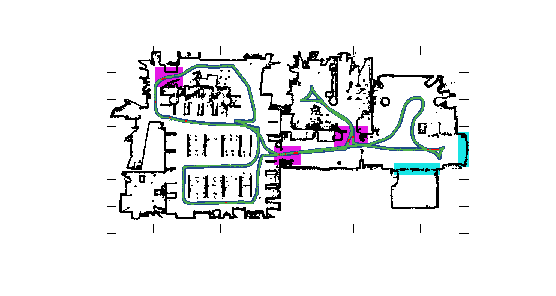
\includegraphics[trim={0 0 0 0.4cm},clip]{./figures/experiments/a/trajectory}}%
    \gplfronttext
  \end{picture}%
\endgroup

  \caption{\small The map of the CSAL environment (black), the trajectory of
           the sensor (blue), CBGL's estimated positions of the sensor (green),
           sensor poses for which CBGL estimated positions with error larger
           than $\delta_{\bm{l}} = 0.5$ m (red), and sources of great range
           noise (purple, cyan). Estimation is performed for each sensor pose
           independently of previous estimates or measurements}
           \label{fig:a:map_and_trajectory}
\end{figure}

\begin{figure}
  \definecolor{g1}{RGB}{200 200 200}
\definecolor{g2}{RGB}{162 162 162}
\definecolor{g3}{RGB}{137 137 137}
\definecolor{g4}{RGB}{77 175 74}

% GNUPLOT: LaTeX picture with Postscript
\begingroup
  \makeatletter
  \providecommand\color[2][]{%
    \GenericError{(gnuplot) \space\space\space\@spaces}{%
      Package color not loaded in conjunction with
      terminal option `colourtext'%
    }{See the gnuplot documentation for explanation.%
    }{Either use 'blacktext' in gnuplot or load the package
      color.sty in LaTeX.}%
    \renewcommand\color[2][]{}%
  }%
  \providecommand\includegraphics[2][]{%
    \GenericError{(gnuplot) \space\space\space\@spaces}{%
      Package graphicx or graphics not loaded%
    }{See the gnuplot documentation for explanation.%
    }{The gnuplot epslatex terminal needs graphicx.sty or graphics.sty.}%
    \renewcommand\includegraphics[2][]{}%
  }%
  \providecommand\rotatebox[2]{#2}%
  \@ifundefined{ifGPcolor}{%
    \newif\ifGPcolor
    \GPcolorfalse
  }{}%
  \@ifundefined{ifGPblacktext}{%
    \newif\ifGPblacktext
    \GPblacktexttrue
  }{}%
  % define a \g@addto@macro without @ in the name:
  \let\gplgaddtomacro\g@addto@macro
  % define empty templates for all commands taking text:
  \gdef\gplfronttext{}%
  \gdef\gplfronttext{}%
  \makeatother
  \ifGPblacktext
    % no textcolor at all
    \def\colorrgb#1{}%
    \def\colorgray#1{}%
  \else
    % gray or color?
    \ifGPcolor
      \def\colorrgb#1{\color[rgb]{#1}}%
      \def\colorgray#1{\color[gray]{#1}}%
      \expandafter\def\csname LTw\endcsname{\color{white}}%
      \expandafter\def\csname LTb\endcsname{\color{black}}%
      \expandafter\def\csname LTa\endcsname{\color{black}}%
      \expandafter\def\csname LT0\endcsname{\color[rgb]{1,0,0}}%
      \expandafter\def\csname LT1\endcsname{\color[rgb]{0,1,0}}%
      \expandafter\def\csname LT2\endcsname{\color[rgb]{0,0,1}}%
      \expandafter\def\csname LT3\endcsname{\color[rgb]{1,0,1}}%
      \expandafter\def\csname LT4\endcsname{\color[rgb]{0,1,1}}%
      \expandafter\def\csname LT5\endcsname{\color[rgb]{1,1,0}}%
      \expandafter\def\csname LT6\endcsname{\color[rgb]{0,0,0}}%
      \expandafter\def\csname LT7\endcsname{\color[rgb]{1,0.3,0}}%
      \expandafter\def\csname LT8\endcsname{\color[rgb]{0.5,0.5,0.5}}%
    \else
      % gray
      \def\colorrgb#1{\color{black}}%
      \def\colorgray#1{\color[gray]{#1}}%
      \expandafter\def\csname LTw\endcsname{\color{white}}%
      \expandafter\def\csname LTb\endcsname{\color{black}}%
      \expandafter\def\csname LTa\endcsname{\color{black}}%
      \expandafter\def\csname LT0\endcsname{\color{black}}%
      \expandafter\def\csname LT1\endcsname{\color{black}}%
      \expandafter\def\csname LT2\endcsname{\color{black}}%
      \expandafter\def\csname LT3\endcsname{\color{black}}%
      \expandafter\def\csname LT4\endcsname{\color{black}}%
      \expandafter\def\csname LT5\endcsname{\color{black}}%
      \expandafter\def\csname LT6\endcsname{\color{black}}%
      \expandafter\def\csname LT7\endcsname{\color{black}}%
      \expandafter\def\csname LT8\endcsname{\color{black}}%
    \fi
  \fi
    \setlength{\unitlength}{0.0500bp}%
    \ifx\gptboxheight\undefined%
      \newlength{\gptboxheight}%
      \newlength{\gptboxwidth}%
      \newsavebox{\gptboxtext}%
    \fi%
    \setlength{\fboxrule}{0.5pt}%
    \setlength{\fboxsep}{1pt}%
\begin{picture}(5000.00,2500.00)%
    \gplgaddtomacro\gplfronttext{%
      \colorrgb{0.15,0.15,0.15}%
      \put(1000,2600){\makebox(0,0){\strut{}{\color{g4}{\rule[0.6mm]{0.5cm}{0.5mm}}} \footnotesize Output}}
      \put(2500,2600){\makebox(0,0){\strut{}{\color{g3}{\rule[0.6mm]{0.5cm}{0.5mm}}} \footnotesize $\mathcal{H}_1[\arg \min f_{\psi}^{\bm{M}}(\mathcal{H}_2)]$}}
      \put(3900,2600){\makebox(0,0){\strut{}{\color{g2}{\rule[0.6mm]{0.5cm}{0.5mm}}} \footnotesize $\mathcal{H}_1$}}
      \put(4500,2600){\makebox(0,0){\strut{}{\color{g1}{\rule[0.6mm]{0.5cm}{0.5mm}}} \footnotesize $\mathcal{H}$}}
      \put(468,250){\makebox(0,0)[r]{\strut{}\footnotesize $0.0$}}%
      \colorrgb{0.15,0.15,0.15}%
      \put(468,750){\makebox(0,0)[r]{\strut{}\footnotesize $0.25$}}%
      \colorrgb{0.15,0.15,0.15}%
      \put(468,1250){\makebox(0,0)[r]{\strut{}\footnotesize $0.50$}}%
      \colorrgb{0.15,0.15,0.15}%
      \put(468,1793){\makebox(0,0)[r]{\strut{}\footnotesize $0.772$}}%
      \colorrgb{0.15,0.15,0.15}%
      \put(468,2105){\makebox(0,0)[r]{\strut{}\footnotesize $0.928$}}%
      \colorrgb{0.15,0.15,0.15}%
      \put(468,2231){\makebox(0,0)[r]{\strut{}\footnotesize $0.991$}}%
      \colorrgb{0.15,0.15,0.15}%
      \put(500,30){\makebox(0,0){\strut{}\footnotesize $5$\texttt{e}-$05$}}%
      \colorrgb{0.15,0.15,0.15}%
      \put(970,30){\makebox(0,0){\strut{}\footnotesize $0.01$}}%
      \colorrgb{0.15,0.15,0.15}%
      \put(1576,30){\makebox(0,0){\strut{}\footnotesize $0.50$}}%
      \colorrgb{0.15,0.15,0.15}%
      %\put(2040,30){\makebox(0,0){\strut{}\footnotesize $10.0$}}%
      \colorrgb{0.15,0.15,0.15}%
      \put(2199,30){\makebox(0,0){\strut{}\footnotesize $27.86$}}%
    }%
    \gplgaddtomacro\gplfronttext{%
      \colorrgb{0.15,0.15,0.15}%
      \put(1349,-300){\makebox(0,0){\strut{}\footnotesize Outliers locational threshold $\delta_{\bm{l}}$ [m]}}%
    }%
    \gplgaddtomacro\gplfronttext{%
      \colorrgb{0.15,0.15,0.15}%
      \put(2893,250){\makebox(0,0)[r]{\strut{}\footnotesize $0.0$}}%
      \colorrgb{0.15,0.15,0.15}%
      \put(2893,750){\makebox(0,0)[r]{\strut{}\footnotesize $0.25$}}%
      \colorrgb{0.15,0.15,0.15}%
      \put(2893,999){\makebox(0,0)[r]{\strut{}\footnotesize $0.375$}}%
      \colorrgb{0.15,0.15,0.15}%
      \put(2893,1153){\makebox(0,0)[r]{\strut{}\footnotesize $0.452$}}%
      \colorrgb{0.15,0.15,0.15}%
      \put(2893,2137){\makebox(0,0)[r]{\strut{}\footnotesize $0.944$}}%
      \colorrgb{0.15,0.15,0.15}%
      \put(2925,30){\makebox(0,0){\strut{}\footnotesize $4$\texttt{e}-$05$}}%
      \colorrgb{0.15,0.15,0.15}%
      \put(3740,30){\makebox(0,0){\strut{}\footnotesize $\frac{\pi}{1000}$}}%
      \colorrgb{0.15,0.15,0.15}%
      \put(4114,30){\makebox(0,0){\strut{}\footnotesize $\frac{\pi}{100}$}}%
      \colorrgb{0.15,0.15,0.15}%
      \put(4749,30){\makebox(0,0){\strut{}\footnotesize $\pi$}}%
    }%
    \gplgaddtomacro\gplfronttext{%
      \colorrgb{0.15,0.15,0.15}%
      \put(3837,-300){\makebox(0,0){\strut{}\footnotesize Outliers angular threshold $\delta_{\alpha}$ [rad]}}%
    }%
    \put(0,0){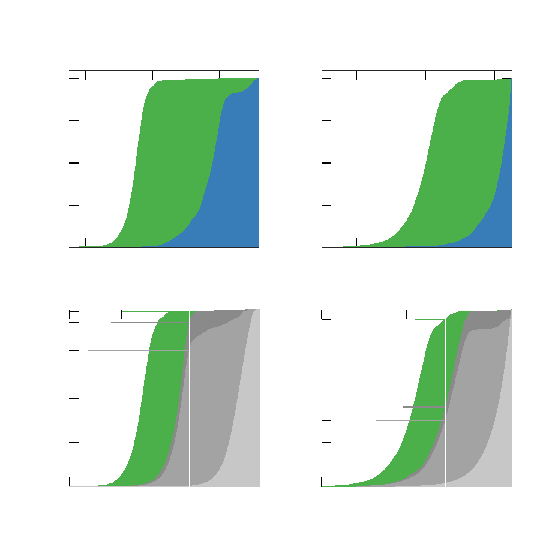
\includegraphics{./figures/experiments/a/awesomeness}}%
    \gplfronttext
  \end{picture}%
\endgroup

  \vspace{0.1cm}
  \caption{\small Proportions of pose estimates whose
           position and orientation error is lower than corresponding thresholds
           $\delta_{\bm{l}}$ and $\delta_{\theta}$. Top: ALS vs CBGL. Bottom:
           CBGL and internal pose estimate sets; the improvement in position
           and orientation induced by scan--to--map-scan matching is captured
           by the difference between the output (i.e.
           $\mathcal{H}_2[\arg \min f_{\psi}^{\bm{M}}(\mathcal{H}_2)]$) and
           $\mathcal{H}_1[\arg \min f_{\psi}^{\bm{M}}(\mathcal{H}_2)]$}
  \label{fig:a:awesomeness}
\end{figure}


\subsection{Simulations against sources of uncertainty}

\begin{figure}\hspace{0.5cm}
  \definecolor{c1}{RGB}{228,26,28}
\definecolor{c2}{RGB}{55,126,184}
\definecolor{c3}{RGB}{255,0,255}
\definecolor{c4}{RGB}{152,78,163}
\definecolor{c5}{RGB}{255,127,0}
\definecolor{c6}{RGB}{77,175,74}
\hspace{0.5cm}

% GNUPLOT: LaTeX picture with Postscript
\begingroup
  \makeatletter
  \providecommand\color[2][]{%
    \GenericError{(gnuplot) \space\space\space\@spaces}{%
      Package color not loaded in conjunction with
      terminal option `colourtext'%
    }{See the gnuplot documentation for explanation.%
    }{Either use 'blacktext' in gnuplot or load the package
      color.sty in LaTeX.}%
    \renewcommand\color[2][]{}%
  }%
  \providecommand\includegraphics[2][]{%
    \GenericError{(gnuplot) \space\space\space\@spaces}{%
      Package graphicx or graphics not loaded%
    }{See the gnuplot documentation for explanation.%
    }{The gnuplot epslatex terminal needs graphicx.sty or graphics.sty.}%
    \renewcommand\includegraphics[2][]{}%
  }%
  \providecommand\rotatebox[2]{#2}%
  \@ifundefined{ifGPcolor}{%
    \newif\ifGPcolor
    \GPcolorfalse
  }{}%
  \@ifundefined{ifGPblacktext}{%
    \newif\ifGPblacktext
    \GPblacktexttrue
  }{}%
  % define a \g@addto@macro without @ in the name:
  \let\gplgaddtomacro\g@addto@macro
  % define empty templates for all commands taking text:
  \gdef\gplfronttext{}%
  \gdef\gplfronttext{}%
  \makeatother
  \ifGPblacktext
    % no textcolor at all
    \def\colorrgb#1{}%
    \def\colorgray#1{}%
  \else
    % gray or color?
    \ifGPcolor
      \def\colorrgb#1{\color[rgb]{#1}}%
      \def\colorgray#1{\color[gray]{#1}}%
      \expandafter\def\csname LTw\endcsname{\color{white}}%
      \expandafter\def\csname LTb\endcsname{\color{black}}%
      \expandafter\def\csname LTa\endcsname{\color{black}}%
      \expandafter\def\csname LT0\endcsname{\color[rgb]{1,0,0}}%
      \expandafter\def\csname LT1\endcsname{\color[rgb]{0,1,0}}%
      \expandafter\def\csname LT2\endcsname{\color[rgb]{0,0,1}}%
      \expandafter\def\csname LT3\endcsname{\color[rgb]{1,0,1}}%
      \expandafter\def\csname LT4\endcsname{\color[rgb]{0,1,1}}%
      \expandafter\def\csname LT5\endcsname{\color[rgb]{1,1,0}}%
      \expandafter\def\csname LT6\endcsname{\color[rgb]{0,0,0}}%
      \expandafter\def\csname LT7\endcsname{\color[rgb]{1,0.3,0}}%
      \expandafter\def\csname LT8\endcsname{\color[rgb]{0.5,0.5,0.5}}%
    \else
      % gray
      \def\colorrgb#1{\color{black}}%
      \def\colorgray#1{\color[gray]{#1}}%
      \expandafter\def\csname LTw\endcsname{\color{white}}%
      \expandafter\def\csname LTb\endcsname{\color{black}}%
      \expandafter\def\csname LTa\endcsname{\color{black}}%
      \expandafter\def\csname LT0\endcsname{\color{black}}%
      \expandafter\def\csname LT1\endcsname{\color{black}}%
      \expandafter\def\csname LT2\endcsname{\color{black}}%
      \expandafter\def\csname LT3\endcsname{\color{black}}%
      \expandafter\def\csname LT4\endcsname{\color{black}}%
      \expandafter\def\csname LT5\endcsname{\color{black}}%
      \expandafter\def\csname LT6\endcsname{\color{black}}%
      \expandafter\def\csname LT7\endcsname{\color{black}}%
      \expandafter\def\csname LT8\endcsname{\color{black}}%
    \fi
  \fi
    \setlength{\unitlength}{0.0500bp}%
    \ifx\gptboxheight\undefined%
      \newlength{\gptboxheight}%
      \newlength{\gptboxwidth}%
      \newsavebox{\gptboxtext}%
    \fi%
    \setlength{\fboxrule}{0.5pt}%
    \setlength{\fboxsep}{1pt}%
  \hspace{0.5cm}
\begin{picture}(5000.00,3000.00)%
    \gplgaddtomacro\gplfronttext{%
      \colorrgb{0.15,0.15,0.15}%
      \put(368,1724){\makebox(0,0)[r]{\strut{}\footnotesize $0\%$}}%
      \colorrgb{0.15,0.15,0.15}%
      \put(368,1968){\makebox(0,0)[r]{\strut{}\footnotesize $25\%$}}%
      \colorrgb{0.15,0.15,0.15}%
      \put(368,2212){\makebox(0,0)[r]{\strut{}\footnotesize $50\%$}}%
      \colorrgb{0.15,0.15,0.15}%
      \put(368,2455){\makebox(0,0)[r]{\strut{}\footnotesize $75\%$}}%
      \colorrgb{0.15,0.15,0.15}%
      \put(368,2699){\makebox(0,0)[r]{\strut{}\footnotesize $100\%$}}%
      \colorrgb{0.15,0.15,0.15}%
      \put(833,1504){\makebox(0,0){\strut{}\footnotesize $\bm{p}_a^W$}}%
      \colorrgb{0.15,0.15,0.15}%
      \put(1500,1504){\makebox(0,0){\strut{}\footnotesize $\bm{p}_b^W$}}%
      \colorrgb{0.15,0.15,0.15}%
      \put(2166,1504){\makebox(0,0){\strut{}\footnotesize $\bm{p}_c^W$}}%
      \colorrgb{0.15,0.15,0.15}%
      \put(2833,1504){\makebox(0,0){\strut{}\footnotesize $\bm{p}_d^W$}}%
      \colorrgb{0.15,0.15,0.15}%
      \put(3499,1504){\makebox(0,0){\strut{}\footnotesize $\bm{p}_f^W$}}%
      \colorrgb{0.15,0.15,0.15}%
      \put(4166,1504){\makebox(0,0){\strut{}\footnotesize $\bm{p}_g^W$}}%
    }%
    \gplgaddtomacro\gplfronttext{%
      \colorrgb{0.15,0.15,0.15}%
      \put(-198,2211){\rotatebox{90}{\makebox(0,0){\strut{}\footnotesize WAREHOUSE}}}%
      \put( 200,3000){\makebox(0,0){\strut{}{\color{c1}{\rule[0.6mm]{0.3cm}{0.5mm}}} \scriptsize MCL}}
      \put( 800,3000){\makebox(0,0){\strut{}{\color{c2}{\rule[0.6mm]{0.3cm}{0.5mm}}} \scriptsize ALS}}
      \put(1450,3000){\makebox(0,0){\strut{}{\color{c3}{\rule[0.6mm]{0.3cm}{0.5mm}}} \scriptsize GMCL}}
      \put(2300,3000){\makebox(0,0){\strut{}{\color{c4}{\rule[0.6mm]{0.3cm}{0.5mm}}} \scriptsize PGL-FMIC}}
      \put(3300,3000){\makebox(0,0){\strut{}{\color{c5}{\rule[0.6mm]{0.3cm}{0.5mm}}} \scriptsize PGL-PLICP}}
      \put(4250,3000){\makebox(0,0){\strut{}{\color{c6}{\rule[0.6mm]{0.3cm}{0.5mm}}} \scriptsize CBGL}}
    }%
    \gplgaddtomacro\gplfronttext{%
      \colorrgb{0.15,0.15,0.15}%
      \put(368,300){\makebox(0,0)[r]{\strut{}\footnotesize $0\%$}}%
      \colorrgb{0.15,0.15,0.15}%
      \put(368,544){\makebox(0,0)[r]{\strut{}\footnotesize $25\%$}}%
      \colorrgb{0.15,0.15,0.15}%
      \put(368,787){\makebox(0,0)[r]{\strut{}\footnotesize $50\%$}}%
      \colorrgb{0.15,0.15,0.15}%
      \put(368,1031){\makebox(0,0)[r]{\strut{}\footnotesize $75\%$}}%
      \colorrgb{0.15,0.15,0.15}%
      \put(368,1274){\makebox(0,0)[r]{\strut{}\footnotesize $100\%$}}%
      \colorrgb{0.15,0.15,0.15}%
      \put(700,80){\makebox(0,0){\strut{}\footnotesize $\bm{p}_a^G$}}%
      \colorrgb{0.15,0.15,0.15}%
      \put(1100,80){\makebox(0,0){\strut{}\footnotesize $\bm{p}_b^G$}}%
      \colorrgb{0.15,0.15,0.15}%
      \put(1500,80){\makebox(0,0){\strut{}\footnotesize $\bm{p}_c^G$}}%
      \colorrgb{0.15,0.15,0.15}%
      \put(1900,80){\makebox(0,0){\strut{}\footnotesize $\bm{p}_d^G$}}%
      \colorrgb{0.15,0.15,0.15}%
      \put(2300,80){\makebox(0,0){\strut{}\footnotesize $\bm{p}_e^G$}}%
      \colorrgb{0.15,0.15,0.15}%
      \put(2699,80){\makebox(0,0){\strut{}\footnotesize $\bm{p}_f^G$}}%
      \colorrgb{0.15,0.15,0.15}%
      \put(3099,80){\makebox(0,0){\strut{}\footnotesize $\bm{p}_g^G$}}%
      \colorrgb{0.15,0.15,0.15}%
      \put(3499,80){\makebox(0,0){\strut{}\footnotesize $\bm{p}_h^G$}}%
      \colorrgb{0.15,0.15,0.15}%
      \put(3899,80){\makebox(0,0){\strut{}\footnotesize $\bm{p}_i^G$}}%
      \colorrgb{0.15,0.15,0.15}%
      \put(4299,80){\makebox(0,0){\strut{}\footnotesize $\bm{p}_j^G$}}%
    }%
    \gplgaddtomacro\gplfronttext{%
      \colorrgb{0.15,0.15,0.15}%
      \put(-198,787){\rotatebox{90}{\makebox(0,0){\strut{}\footnotesize WILLOWGARAGE}}}%
    }%
    \put(0,0){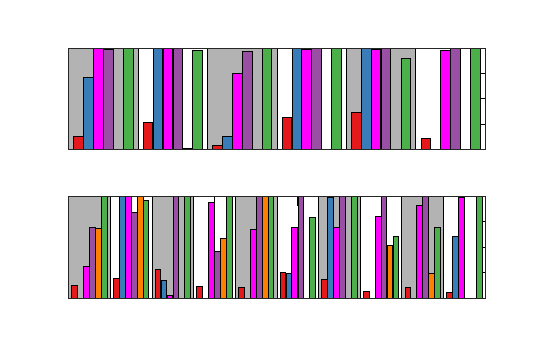
\includegraphics{./figures/experiments/b/inliers_per_pose}}%
    \gplfronttext
  \end{picture}%
\endgroup

  \caption{\small}
  \label{fig:}
\end{figure}
%\begin{figure}
  %\input{./figures/experiments/b/outliers.tex}
  %\caption{\small}
  %\label{fig:}
%\end{figure}
\begin{figure}
  \definecolor{c1}{RGB}{228,26,28}
\definecolor{c2}{RGB}{55,126,184}
\definecolor{c3}{RGB}{255,0,255}
\definecolor{c4}{RGB}{152,78,163}
\definecolor{c5}{RGB}{255,127,0}
\definecolor{c6}{RGB}{77,175,74}

% GNUPLOT: LaTeX picture with Postscript
\begingroup
  \makeatletter
  \providecommand\color[2][]{%
    \GenericError{(gnuplot) \space\space\space\@spaces}{%
      Package color not loaded in conjunction with
      terminal option `colourtext'%
    }{See the gnuplot documentation for explanation.%
    }{Either use 'blacktext' in gnuplot or load the package
      color.sty in LaTeX.}%
    \renewcommand\color[2][]{}%
  }%
  \providecommand\includegraphics[2][]{%
    \GenericError{(gnuplot) \space\space\space\@spaces}{%
      Package graphicx or graphics not loaded%
    }{See the gnuplot documentation for explanation.%
    }{The gnuplot epslatex terminal needs graphicx.sty or graphics.sty.}%
    \renewcommand\includegraphics[2][]{}%
  }%
  \providecommand\rotatebox[2]{#2}%
  \@ifundefined{ifGPcolor}{%
    \newif\ifGPcolor
    \GPcolorfalse
  }{}%
  \@ifundefined{ifGPblacktext}{%
    \newif\ifGPblacktext
    \GPblacktexttrue
  }{}%
  % define a \g@addto@macro without @ in the name:
  \let\gplgaddtomacro\g@addto@macro
  % define empty templates for all commands taking text:
  \gdef\gplfronttext{}%
  \gdef\gplfronttext{}%
  \makeatother
  \ifGPblacktext
    % no textcolor at all
    \def\colorrgb#1{}%
    \def\colorgray#1{}%
  \else
    % gray or color?
    \ifGPcolor
      \def\colorrgb#1{\color[rgb]{#1}}%
      \def\colorgray#1{\color[gray]{#1}}%
      \expandafter\def\csname LTw\endcsname{\color{white}}%
      \expandafter\def\csname LTb\endcsname{\color{black}}%
      \expandafter\def\csname LTa\endcsname{\color{black}}%
      \expandafter\def\csname LT0\endcsname{\color[rgb]{1,0,0}}%
      \expandafter\def\csname LT1\endcsname{\color[rgb]{0,1,0}}%
      \expandafter\def\csname LT2\endcsname{\color[rgb]{0,0,1}}%
      \expandafter\def\csname LT3\endcsname{\color[rgb]{1,0,1}}%
      \expandafter\def\csname LT4\endcsname{\color[rgb]{0,1,1}}%
      \expandafter\def\csname LT5\endcsname{\color[rgb]{1,1,0}}%
      \expandafter\def\csname LT6\endcsname{\color[rgb]{0,0,0}}%
      \expandafter\def\csname LT7\endcsname{\color[rgb]{1,0.3,0}}%
      \expandafter\def\csname LT8\endcsname{\color[rgb]{0.5,0.5,0.5}}%
    \else
      % gray
      \def\colorrgb#1{\color{black}}%
      \def\colorgray#1{\color[gray]{#1}}%
      \expandafter\def\csname LTw\endcsname{\color{white}}%
      \expandafter\def\csname LTb\endcsname{\color{black}}%
      \expandafter\def\csname LTa\endcsname{\color{black}}%
      \expandafter\def\csname LT0\endcsname{\color{black}}%
      \expandafter\def\csname LT1\endcsname{\color{black}}%
      \expandafter\def\csname LT2\endcsname{\color{black}}%
      \expandafter\def\csname LT3\endcsname{\color{black}}%
      \expandafter\def\csname LT4\endcsname{\color{black}}%
      \expandafter\def\csname LT5\endcsname{\color{black}}%
      \expandafter\def\csname LT6\endcsname{\color{black}}%
      \expandafter\def\csname LT7\endcsname{\color{black}}%
      \expandafter\def\csname LT8\endcsname{\color{black}}%
    \fi
  \fi
    \setlength{\unitlength}{0.0500bp}%
    \ifx\gptboxheight\undefined%
      \newlength{\gptboxheight}%
      \newlength{\gptboxwidth}%
      \newsavebox{\gptboxtext}%
    \fi%
    \setlength{\fboxrule}{0.5pt}%
    \setlength{\fboxsep}{1pt}%
\begin{picture}(5000.00,1500.00)%
    \gplgaddtomacro\gplfronttext{%
      \colorrgb{0.15,0.15,0.15}%
      \put(368,267){\makebox(0,0)[r]{\strut{}\footnotesize $10^{0}$}}%
      \colorrgb{0.15,0.15,0.15}%
      \put(368,657){\makebox(0,0)[r]{\strut{}\footnotesize $10^{1}$}}%
      \colorrgb{0.15,0.15,0.15}%
      \put(368,1046){\makebox(0,0)[r]{\strut{}\footnotesize $10^{2}$}}%
    }%
    \gplgaddtomacro\gplfronttext{%
      \colorrgb{0.15,0.15,0.15}%
      \put(1474,-70){\makebox(0,0){\strut{}\footnotesize WAREHOUSE}}%
      \put( 400,1500){\makebox(0,0){\strut{}{\color{c1}{\rule[0.6mm]{0.3cm}{0.5mm}}} \scriptsize MCL}}
      \put(1000,1500){\makebox(0,0){\strut{}{\color{c2}{\rule[0.6mm]{0.3cm}{0.5mm}}} \scriptsize ALS}}
      \put(1650,1500){\makebox(0,0){\strut{}{\color{c3}{\rule[0.6mm]{0.3cm}{0.5mm}}} \scriptsize GMCL}}
      \put(2500,1500){\makebox(0,0){\strut{}{\color{c4}{\rule[0.6mm]{0.3cm}{0.5mm}}} \scriptsize PGL-FMIC}}
      \put(3500,1500){\makebox(0,0){\strut{}{\color{c5}{\rule[0.6mm]{0.3cm}{0.5mm}}} \scriptsize PGL-PLICP}}
      \put(4450,1500){\makebox(0,0){\strut{}{\color{c6}{\rule[0.6mm]{0.3cm}{0.5mm}}} \scriptsize CBGL}}
    }%
    \gplgaddtomacro\gplfronttext{%
      \colorrgb{0.15,0.15,0.15}%
      \put(2418,267){\makebox(0,0)[r]{\strut{}\footnotesize $10^{0}$}}%
      \colorrgb{0.15,0.15,0.15}%
      \put(2418,657){\makebox(0,0)[r]{\strut{}\footnotesize $10^{1}$}}%
      \colorrgb{0.15,0.15,0.15}%
      \put(2418,1046){\makebox(0,0)[r]{\strut{}\footnotesize $10^{2}$}}%
    }%
    \gplgaddtomacro\gplfronttext{%
      \colorrgb{0.15,0.15,0.15}%
      \put(3524,-70){\makebox(0,0){\strut{}\footnotesize WILLOWGARAGE}}%
    }%
    \put(0,0){\includegraphics{./figures/experiments/b/exec_times}}%
    \gplfronttext
  \end{picture}%
\endgroup

  \caption{\small}
  \label{fig:}
\end{figure}


\subsection{Simulations against environment disparity and choice of scan--to--map-scan matching methods}
\begin{figure}
  % GNUPLOT: LaTeX picture with Postscript
\begingroup
  \makeatletter
  \providecommand\color[2][]{%
    \GenericError{(gnuplot) \space\space\space\@spaces}{%
      Package color not loaded in conjunction with
      terminal option `colourtext'%
    }{See the gnuplot documentation for explanation.%
    }{Either use 'blacktext' in gnuplot or load the package
      color.sty in LaTeX.}%
    \renewcommand\color[2][]{}%
  }%
  \providecommand\includegraphics[2][]{%
    \GenericError{(gnuplot) \space\space\space\@spaces}{%
      Package graphicx or graphics not loaded%
    }{See the gnuplot documentation for explanation.%
    }{The gnuplot epslatex terminal needs graphicx.sty or graphics.sty.}%
    \renewcommand\includegraphics[2][]{}%
  }%
  \providecommand\rotatebox[2]{#2}%
  \@ifundefined{ifGPcolor}{%
    \newif\ifGPcolor
    \GPcolorfalse
  }{}%
  \@ifundefined{ifGPblacktext}{%
    \newif\ifGPblacktext
    \GPblacktexttrue
  }{}%
  % define a \g@addto@macro without @ in the name:
  \let\gplgaddtomacro\g@addto@macro
  % define empty templates for all commands taking text:
  \gdef\gplfronttext{}%
  \gdef\gplfronttext{}%
  \makeatother
  \ifGPblacktext
    % no textcolor at all
    \def\colorrgb#1{}%
    \def\colorgray#1{}%
  \else
    % gray or color?
    \ifGPcolor
      \def\colorrgb#1{\color[rgb]{#1}}%
      \def\colorgray#1{\color[gray]{#1}}%
      \expandafter\def\csname LTw\endcsname{\color{white}}%
      \expandafter\def\csname LTb\endcsname{\color{black}}%
      \expandafter\def\csname LTa\endcsname{\color{black}}%
      \expandafter\def\csname LT0\endcsname{\color[rgb]{1,0,0}}%
      \expandafter\def\csname LT1\endcsname{\color[rgb]{0,1,0}}%
      \expandafter\def\csname LT2\endcsname{\color[rgb]{0,0,1}}%
      \expandafter\def\csname LT3\endcsname{\color[rgb]{1,0,1}}%
      \expandafter\def\csname LT4\endcsname{\color[rgb]{0,1,1}}%
      \expandafter\def\csname LT5\endcsname{\color[rgb]{1,1,0}}%
      \expandafter\def\csname LT6\endcsname{\color[rgb]{0,0,0}}%
      \expandafter\def\csname LT7\endcsname{\color[rgb]{1,0.3,0}}%
      \expandafter\def\csname LT8\endcsname{\color[rgb]{0.5,0.5,0.5}}%
    \else
      % gray
      \def\colorrgb#1{\color{black}}%
      \def\colorgray#1{\color[gray]{#1}}%
      \expandafter\def\csname LTw\endcsname{\color{white}}%
      \expandafter\def\csname LTb\endcsname{\color{black}}%
      \expandafter\def\csname LTa\endcsname{\color{black}}%
      \expandafter\def\csname LT0\endcsname{\color{black}}%
      \expandafter\def\csname LT1\endcsname{\color{black}}%
      \expandafter\def\csname LT2\endcsname{\color{black}}%
      \expandafter\def\csname LT3\endcsname{\color{black}}%
      \expandafter\def\csname LT4\endcsname{\color{black}}%
      \expandafter\def\csname LT5\endcsname{\color{black}}%
      \expandafter\def\csname LT6\endcsname{\color{black}}%
      \expandafter\def\csname LT7\endcsname{\color{black}}%
      \expandafter\def\csname LT8\endcsname{\color{black}}%
    \fi
  \fi
    \setlength{\unitlength}{0.0500bp}%
    \ifx\gptboxheight\undefined%
      \newlength{\gptboxheight}%
      \newlength{\gptboxwidth}%
      \newsavebox{\gptboxtext}%
    \fi%
    \setlength{\fboxrule}{0.5pt}%
    \setlength{\fboxsep}{1pt}%
\begin{picture}(5000.00,2500.00)%
    \gplgaddtomacro\gplfronttext{%
      \colorrgb{0.15,0.15,0.15}%
      \put(368,250){\makebox(0,0)[r]{\strut{}0}}%
      \colorrgb{0.15,0.15,0.15}%
      \put(368,650){\makebox(0,0)[r]{\strut{}0.2}}%
      \colorrgb{0.15,0.15,0.15}%
      \put(368,1050){\makebox(0,0)[r]{\strut{}0.4}}%
      \colorrgb{0.15,0.15,0.15}%
      \put(368,1449){\makebox(0,0)[r]{\strut{}0.6}}%
      \colorrgb{0.15,0.15,0.15}%
      \put(368,1849){\makebox(0,0)[r]{\strut{}0.8}}%
      \colorrgb{0.15,0.15,0.15}%
      \put(368,2249){\makebox(0,0)[r]{\strut{}1}}%
      \colorrgb{0.15,0.15,0.15}%
      \put(826,30){\makebox(0,0){\strut{}$10^{-2}$}}%
      \colorrgb{0.15,0.15,0.15}%
      \put(1200,30){\makebox(0,0){\strut{}$10^{-1}$}}%
      \colorrgb{0.15,0.15,0.15}%
      \put(1575,30){\makebox(0,0){\strut{}$10^{0}$}}%
      \colorrgb{0.15,0.15,0.15}%
      \put(1949,30){\makebox(0,0){\strut{}$10^{1}$}}%
      \colorrgb{0.15,0.15,0.15}%
      \put(2323,30){\makebox(0,0){\strut{}$10^{2}$}}%
    }%
    \gplgaddtomacro\gplfronttext{%
    }%
    \gplgaddtomacro\gplfronttext{%
      \colorrgb{0.15,0.15,0.15}%
      \put(2493,250){\makebox(0,0)[r]{\strut{}0}}%
      \colorrgb{0.15,0.15,0.15}%
      \put(2493,650){\makebox(0,0)[r]{\strut{}0.2}}%
      \colorrgb{0.15,0.15,0.15}%
      \put(2493,1050){\makebox(0,0)[r]{\strut{}0.4}}%
      \colorrgb{0.15,0.15,0.15}%
      \put(2493,1449){\makebox(0,0)[r]{\strut{}0.6}}%
      \colorrgb{0.15,0.15,0.15}%
      \put(2493,1849){\makebox(0,0)[r]{\strut{}0.8}}%
      \colorrgb{0.15,0.15,0.15}%
      \put(2493,2249){\makebox(0,0)[r]{\strut{}1}}%
      \colorrgb{0.15,0.15,0.15}%
      \put(2813,30){\makebox(0,0){\strut{}$10^{-4}$}}%
      \colorrgb{0.15,0.15,0.15}%
      \put(3188,30){\makebox(0,0){\strut{}$10^{-3}$}}%
      \colorrgb{0.15,0.15,0.15}%
      \put(3563,30){\makebox(0,0){\strut{}$10^{-2}$}}%
      \colorrgb{0.15,0.15,0.15}%
      \put(3938,30){\makebox(0,0){\strut{}$10^{-1}$}}%
      \colorrgb{0.15,0.15,0.15}%
      \put(4313,30){\makebox(0,0){\strut{}$10^{0}$}}%
    }%
    \gplgaddtomacro\gplfronttext{%
    }%
    \put(0,0){
\includegraphics{./figures/experiments/c/awesome}}%
    \gplfronttext
  \end{picture}%
\endgroup

  \caption{\small}
  \label{fig:}
\end{figure}
\begin{figure}
  \definecolor{c0}{RGB}{162 162 162}
\definecolor{c1}{RGB}{102 194 165}
\definecolor{c2}{RGB}{252 141 98}
\definecolor{c3}{RGB}{41 160 203}
\definecolor{c4}{RGB}{231 138 195}

% GNUPLOT: LaTeX picture with Postscript
\begingroup
  \makeatletter
  \providecommand\color[2][]{%
    \GenericError{(gnuplot) \space\space\space\@spaces}{%
      Package color not loaded in conjunction with
      terminal option `colourtext'%
    }{See the gnuplot documentation for explanation.%
    }{Either use 'blacktext' in gnuplot or load the package
      color.sty in LaTeX.}%
    \renewcommand\color[2][]{}%
  }%
  \providecommand\includegraphics[2][]{%
    \GenericError{(gnuplot) \space\space\space\@spaces}{%
      Package graphicx or graphics not loaded%
    }{See the gnuplot documentation for explanation.%
    }{The gnuplot epslatex terminal needs graphicx.sty or graphics.sty.}%
    \renewcommand\includegraphics[2][]{}%
  }%
  \providecommand\rotatebox[2]{#2}%
  \@ifundefined{ifGPcolor}{%
    \newif\ifGPcolor
    \GPcolorfalse
  }{}%
  \@ifundefined{ifGPblacktext}{%
    \newif\ifGPblacktext
    \GPblacktexttrue
  }{}%
  % define a \g@addto@macro without @ in the name:
  \let\gplgaddtomacro\g@addto@macro
  % define empty templates for all commands taking text:
  \gdef\gplfronttext{}%
  \gdef\gplfronttext{}%
  \makeatother
  \ifGPblacktext
    % no textcolor at all
    \def\colorrgb#1{}%
    \def\colorgray#1{}%
  \else
    % gray or color?
    \ifGPcolor
      \def\colorrgb#1{\color[rgb]{#1}}%
      \def\colorgray#1{\color[gray]{#1}}%
      \expandafter\def\csname LTw\endcsname{\color{white}}%
      \expandafter\def\csname LTb\endcsname{\color{black}}%
      \expandafter\def\csname LTa\endcsname{\color{black}}%
      \expandafter\def\csname LT0\endcsname{\color[rgb]{1,0,0}}%
      \expandafter\def\csname LT1\endcsname{\color[rgb]{0,1,0}}%
      \expandafter\def\csname LT2\endcsname{\color[rgb]{0,0,1}}%
      \expandafter\def\csname LT3\endcsname{\color[rgb]{1,0,1}}%
      \expandafter\def\csname LT4\endcsname{\color[rgb]{0,1,1}}%
      \expandafter\def\csname LT5\endcsname{\color[rgb]{1,1,0}}%
      \expandafter\def\csname LT6\endcsname{\color[rgb]{0,0,0}}%
      \expandafter\def\csname LT7\endcsname{\color[rgb]{1,0.3,0}}%
      \expandafter\def\csname LT8\endcsname{\color[rgb]{0.5,0.5,0.5}}%
    \else
      % gray
      \def\colorrgb#1{\color{black}}%
      \def\colorgray#1{\color[gray]{#1}}%
      \expandafter\def\csname LTw\endcsname{\color{white}}%
      \expandafter\def\csname LTb\endcsname{\color{black}}%
      \expandafter\def\csname LTa\endcsname{\color{black}}%
      \expandafter\def\csname LT0\endcsname{\color{black}}%
      \expandafter\def\csname LT1\endcsname{\color{black}}%
      \expandafter\def\csname LT2\endcsname{\color{black}}%
      \expandafter\def\csname LT3\endcsname{\color{black}}%
      \expandafter\def\csname LT4\endcsname{\color{black}}%
      \expandafter\def\csname LT5\endcsname{\color{black}}%
      \expandafter\def\csname LT6\endcsname{\color{black}}%
      \expandafter\def\csname LT7\endcsname{\color{black}}%
      \expandafter\def\csname LT8\endcsname{\color{black}}%
    \fi
  \fi
    \setlength{\unitlength}{0.0500bp}%
    \ifx\gptboxheight\undefined%
      \newlength{\gptboxheight}%
      \newlength{\gptboxwidth}%
      \newsavebox{\gptboxtext}%
    \fi%
    \setlength{\fboxrule}{0.5pt}%
    \setlength{\fboxsep}{1pt}%
\begin{picture}(5000.00,1500.00)%
    \gplgaddtomacro\gplfronttext{%
      \colorrgb{0.15,0.15,0.15}%
      \put(468,224){\makebox(0,0)[r]{\strut{}\scriptsize $10^{-4}$}}%
      \colorrgb{0.15,0.15,0.15}%
      \put(468,468){\makebox(0,0)[r]{\strut{}\scriptsize $10^{-3}$}}%
      \colorrgb{0.15,0.15,0.15}%
      \put(468,713){\makebox(0,0)[r]{\strut{}\scriptsize $10^{-2}$}}%
      \colorrgb{0.15,0.15,0.15}%
      \put(468,957){\makebox(0,0)[r]{\strut{}\scriptsize $10^{-1}$}}%
      \colorrgb{0.15,0.15,0.15}%
      \put(368,1202){\makebox(0,0)[r]{\strut{}\scriptsize $10^{0}$}}%
    }%
    \gplgaddtomacro\gplfronttext{%
      \colorrgb{0.15,0.15,0.15}%
      \put(999,-70){\makebox(0,0){\strut{}\scriptsize Position errors [m]}}%
      \put( 800,1500){\makebox(0,0){\strut{}{\color{c0}{\rule[0.6mm]{0.3cm}{0.5mm}}} \scriptsize $\mathcal{H}_1$}}
      \put( 1400,1500){\makebox(0,0){\strut{}{\color{c1}{\rule[0.6mm]{0.3cm}{0.5mm}}} \scriptsize NDT}}
      \put(2300,1500){\makebox(0,0){\strut{}{\color{c2}{\rule[0.6mm]{0.3cm}{0.5mm}}} \scriptsize FastGICP}}
      \put(3400,1500){\makebox(0,0){\strut{}{\color{c3}{\rule[0.6mm]{0.3cm}{0.5mm}}} \scriptsize FastVGICP}}
      \put(4200,1500){\makebox(0,0){\strut{}{\color{c4}{\rule[0.6mm]{0.3cm}{0.5mm}}} \scriptsize \texttt{x1}}}
    }%
    \gplgaddtomacro\gplfronttext{%
      \colorrgb{0.15,0.15,0.15}%
      \put(1968,210){\makebox(0,0)[r]{\strut{}\scriptsize $10^{-4}$}}%
      \colorrgb{0.15,0.15,0.15}%
      \put(1968,410){\makebox(0,0)[r]{\strut{}\scriptsize $10^{-5}$}}%
      \colorrgb{0.15,0.15,0.15}%
      \put(1968,610){\makebox(0,0)[r]{\strut{}\scriptsize $10^{-3}$}}%
      \colorrgb{0.15,0.15,0.15}%
      \put(1968,810){\makebox(0,0)[r]{\strut{}\scriptsize $10^{-2}$}}%
      \colorrgb{0.15,0.15,0.15}%
      \put(1968,1009){\makebox(0,0)[r]{\strut{}\scriptsize $10^{-1}$}}%
      \colorrgb{0.15,0.15,0.15}%
      \put(1868,1209){\makebox(0,0)[r]{\strut{}\scriptsize $10^{0}$}}%
    }%
    \gplgaddtomacro\gplfronttext{%
      \colorrgb{0.15,0.15,0.15}%
      \put(2499,-70){\makebox(0,0){\strut{}\scriptsize Orientation errors [rad]}}%
    }%
    \gplgaddtomacro\gplfronttext{%
      \colorrgb{0.15,0.15,0.15}%
      \put(3468,150){\makebox(0,0)[r]{\strut{}\scriptsize $0.0$}}%
      \colorrgb{0.15,0.15,0.15}%
      \put(3468,450){\makebox(0,0)[r]{\strut{}\scriptsize $2.0$}}%
      \colorrgb{0.15,0.15,0.15}%
      \put(3468,750){\makebox(0,0)[r]{\strut{}\scriptsize $4.0$}}%
      \colorrgb{0.15,0.15,0.15}%
      \put(3468,1049){\makebox(0,0)[r]{\strut{}\scriptsize $6.0$}}%
      \colorrgb{0.15,0.15,0.15}%
      \put(3468,1349){\makebox(0,0)[r]{\strut{}\scriptsize $8.0$}}%
    }%
    \gplgaddtomacro\gplfronttext{%
      \colorrgb{0.15,0.15,0.15}%
      \put(3999,-70){\makebox(0,0){\strut{}\scriptsize Execution times [sec]}}%
    }%
    \put(0,0){\includegraphics{./figures/experiments/c/errors}}%
    \gplfronttext
  \end{picture}%
\endgroup

  \caption{\small}
  \label{fig:}
\end{figure}



%%%%%%%%%%%%%%%%%%%%%%%%%%%%%%%%%%%%%%%%%%%%%%%%%%%%%%%%%%%%%%%%%%%%%%%%%%%%%%%%
\section{Characterisation}
  \label{section:characterisation}
  Range scans with panoramic angular ranges induce fewer pose ambiguities in
rank-fields than those with non-panoramic field of view. In the latter case
this means that, given the evidence of subsections \ref{subsec:exp_a} and
\ref{subsec:exp_c} where $\lambda = 3\pi/2$ rad, the choice of $k=10$ largely
inhibits the propagation of ambiguities to the output (fig.
\ref{fig:c:errors_and_time}).  However, non-panoramic sensors coupled
with repeated environment structures may give rise to the conditions of figure
\ref{fig:h_and_h_not_fig} (bottom). Other sources of potential, large pose
errors for CBGL are portrayed in figure \ref{fig:a:map_and_trajectory}: (a)
regions coloured with cyan indicate closed glass doors, wherein high range
errors result in discrepancy with map-derived virtual ranges, which is
subsequently propagated to $\psi$-fields and hence $\texttt{r}$-fields, and (b)
regions coloured purple indicate vicinities around doors, wherein
higher locational density or values of $k$ may be required to suppress pose
ambiguities propagated to $\texttt{r}$-fields.

\begin{figure}
  \definecolor{v}{RGB}{131, 186, 109}
\definecolor{x}{RGB}{217, 33, 32}
\definecolor{w}{RGB}{120, 28, 130}

% GNUPLOT: LaTeX picture with Postscript
\begingroup
  \makeatletter
  \providecommand\color[2][]{%
    \GenericError{(gnuplot) \space\space\space\@spaces}{%
      Package color not loaded in conjunction with
      terminal option `colourtext'%
    }{See the gnuplot documentation for explanation.%
    }{Either use 'blacktext' in gnuplot or load the package
      color.sty in LaTeX.}%
    \renewcommand\color[2][]{}%
  }%
  \providecommand\includegraphics[2][]{%
    \GenericError{(gnuplot) \space\space\space\@spaces}{%
      Package graphicx or graphics not loaded%
    }{See the gnuplot documentation for explanation.%
    }{The gnuplot epslatex terminal needs graphicx.sty or graphics.sty.}%
    \renewcommand\includegraphics[2][]{}%
  }%
  \providecommand\rotatebox[2]{#2}%
  \@ifundefined{ifGPcolor}{%
    \newif\ifGPcolor
    \GPcolorfalse
  }{}%
  \@ifundefined{ifGPblacktext}{%
    \newif\ifGPblacktext
    \GPblacktexttrue
  }{}%
  % define a \g@addto@macro without @ in the name:
  \let\gplgaddtomacro\g@addto@macro
  % define empty templates for all commands taking text:
  \gdef\gplfronttext{}%
  \gdef\gplfronttext{}%
  \makeatother
  \ifGPblacktext
    % no textcolor at all
    \def\colorrgb#1{}%
    \def\colorgray#1{}%
  \else
    % gray or color?
    \ifGPcolor
      \def\colorrgb#1{\color[rgb]{#1}}%
      \def\colorgray#1{\color[gray]{#1}}%
      \expandafter\def\csname LTw\endcsname{\color{white}}%
      \expandafter\def\csname LTb\endcsname{\color{black}}%
      \expandafter\def\csname LTa\endcsname{\color{black}}%
      \expandafter\def\csname LT0\endcsname{\color[rgb]{1,0,0}}%
      \expandafter\def\csname LT1\endcsname{\color[rgb]{0,1,0}}%
      \expandafter\def\csname LT2\endcsname{\color[rgb]{0,0,1}}%
      \expandafter\def\csname LT3\endcsname{\color[rgb]{1,0,1}}%
      \expandafter\def\csname LT4\endcsname{\color[rgb]{0,1,1}}%
      \expandafter\def\csname LT5\endcsname{\color[rgb]{1,1,0}}%
      \expandafter\def\csname LT6\endcsname{\color[rgb]{0,0,0}}%
      \expandafter\def\csname LT7\endcsname{\color[rgb]{1,0.3,0}}%
      \expandafter\def\csname LT8\endcsname{\color[rgb]{0.5,0.5,0.5}}%
    \else
      % gray
      \def\colorrgb#1{\color{black}}%
      \def\colorgray#1{\color[gray]{#1}}%
      \expandafter\def\csname LTw\endcsname{\color{white}}%
      \expandafter\def\csname LTb\endcsname{\color{black}}%
      \expandafter\def\csname LTa\endcsname{\color{black}}%
      \expandafter\def\csname LT0\endcsname{\color{black}}%
      \expandafter\def\csname LT1\endcsname{\color{black}}%
      \expandafter\def\csname LT2\endcsname{\color{black}}%
      \expandafter\def\csname LT3\endcsname{\color{black}}%
      \expandafter\def\csname LT4\endcsname{\color{black}}%
      \expandafter\def\csname LT5\endcsname{\color{black}}%
      \expandafter\def\csname LT6\endcsname{\color{black}}%
      \expandafter\def\csname LT7\endcsname{\color{black}}%
      \expandafter\def\csname LT8\endcsname{\color{black}}%
    \fi
  \fi
    \setlength{\unitlength}{0.0500bp}%
    \ifx\gptboxheight\undefined%
      \newlength{\gptboxheight}%
      \newlength{\gptboxwidth}%
      \newsavebox{\gptboxtext}%
    \fi%
    \setlength{\fboxrule}{0.5pt}%
    \setlength{\fboxsep}{1pt}%

\hspace{0.25cm}
\begin{picture}(4600.00,3500.00)%
    \gplgaddtomacro\gplfronttext{%
      \colorrgb{0.15,0.15,0.15}%
      \put(428,1925){\makebox(0,0)[r]{\strut{}\footnotesize $0$}}%
      \colorrgb{0.15,0.15,0.15}%
      \put(428,2129){\makebox(0,0)[r]{\strut{}\footnotesize $\psi_0$}}%
      \colorrgb{0.15,0.15,0.15}%
      \put(428,2333){\makebox(0,0)[r]{\strut{}\footnotesize $400$}}%
      \colorrgb{0.15,0.15,0.15}%
      \put(428,2741){\makebox(0,0)[r]{\strut{}\footnotesize $800$}}%
      \colorrgb{0.15,0.15,0.15}%
      \put(428,3149){\makebox(0,0)[r]{\strut{}\footnotesize $1200$}}%
      \colorrgb{0.15,0.15,0.15}%
      \put(460,1755){\makebox(0,0){\strut{}\footnotesize $0.05$}}%
      \colorrgb{0.15,0.15,0.15}%
      \put(1378,1755){\makebox(0,0){\strut{}\footnotesize $\delta_0$}}%
      \colorrgb{0.15,0.15,0.15}%
      \put(1659,1755){\makebox(0,0){\strut{}\footnotesize $1.5$}}%
      \colorrgb{0.15,0.15,0.15}%
      %\put(1903,2705){\makebox(0,0){\strut{}\footnotesize $3.0$}}%
      \colorrgb{0.15,0.15,0.15}%
      \put(2046,1755){\makebox(0,0){\strut{}\footnotesize $4.5$}}%
    }%
    \gplgaddtomacro\gplfronttext{%
      \colorrgb{0.15,0.15,0.15}%
      \put(-150,2537){\rotatebox{90}{\makebox(0,0){\strut{}\footnotesize CAER [m]}}}%
    }%
    \gplgaddtomacro\gplfronttext{%
      \colorrgb{0.15,0.15,0.15}%
      \put(2935,1925){\makebox(0,0)[r]{\strut{}\footnotesize $10^0$}}%
      \colorrgb{0.15,0.15,0.15}%
      \put(2935,2168){\makebox(0,0)[r]{\strut{}\footnotesize $10^1$}}%
      \colorrgb{0.15,0.15,0.15}%
      \put(2935,2411){\makebox(0,0)[r]{\strut{}\footnotesize $10^2$}}%
      \colorrgb{0.15,0.15,0.15}%
      \put(2935,2655){\makebox(0,0)[r]{\strut{}\footnotesize $10^3$}}%
      \colorrgb{0.15,0.15,0.15}%
      \put(2935,2898){\makebox(0,0)[r]{\strut{}\footnotesize $10^4$}}%
      \colorrgb{0.15,0.15,0.15}%
      \put(2935,3141){\makebox(0,0)[r]{\strut{}\footnotesize $10^5$}}%
      \colorrgb{0.15,0.15,0.15}%
      \put(2967,1755){\makebox(0,0){\strut{}\footnotesize $0.05$}}%
      \colorrgb{0.15,0.15,0.15}%
      \put(3885,1755){\makebox(0,0){\strut{}\footnotesize $\delta_0$}}%
      \colorrgb{0.15,0.15,0.15}%
      \put(4166,1755){\makebox(0,0){\strut{}\footnotesize $1.5$}}%
      \colorrgb{0.15,0.15,0.15}%
      %\put(4410,2705){\makebox(0,0){\strut{}\footnotesize $3.0$}}%
      \colorrgb{0.15,0.15,0.15}%
      \put(4553,1755){\makebox(0,0){\strut{}\footnotesize $4.5$}}%
    }%
    \gplgaddtomacro\gplfronttext{%
      \colorrgb{0.15,0.15,0.15}%
      \put(2400,2537){\rotatebox{90}{\makebox(0,0){\strut{}\footnotesize Hypotheses' ranks}}}%
    }%
    \gplgaddtomacro\gplfronttext{%
      \colorrgb{0.15,0.15,0.15}%
      \put(428,441){\makebox(0,0)[r]{\strut{}\footnotesize $\psi_0$}}%
      \colorrgb{0.15,0.15,0.15}%
      \put(428,979){\makebox(0,0)[r]{\strut{}\footnotesize $500$}}%
      \colorrgb{0.15,0.15,0.15}%
      \put(428,1244){\makebox(0,0)[r]{\strut{}\footnotesize $1000$}}%
      \colorrgb{0.15,0.15,0.15}%
      \put(428,1510){\makebox(0,0)[r]{\strut{}\footnotesize $2000$}}%
      \colorrgb{0.15,0.15,0.15}%
      \put(460,180){\makebox(0,0){\strut{}\footnotesize $0.05$}}%
      \colorrgb{0.15,0.15,0.15}%
      \put(854,180){\makebox(0,0){\strut{}\footnotesize $5.0$}}%
      \colorrgb{0.15,0.15,0.15}%
      \put(1251,180){\makebox(0,0){\strut{}\footnotesize $10.0$}}%
      \colorrgb{0.15,0.15,0.15}%
      \put(1635,180){\makebox(0,0){\strut{}\footnotesize $\delta_0$}}%
      \colorrgb{0.15,0.15,0.15}%
      \put(2046,180){\makebox(0,0){\strut{}\footnotesize $20.0$}}%
    }%
    \gplgaddtomacro\gplfronttext{%
      \colorrgb{0.15,0.15,0.15}%
      \put(-150,962){\rotatebox{90}{\makebox(0,0){\strut{}\footnotesize CAER [m]}}}%
    }%
    \gplgaddtomacro\gplfronttext{%
      \colorrgb{0.15,0.15,0.15}%
      \put(2935,350){\makebox(0,0)[r]{\strut{}\footnotesize $10^0$}}%
      \colorrgb{0.15,0.15,0.15}%
      \put(2935,554){\makebox(0,0)[r]{\strut{}\footnotesize $10^1$}}%
      \colorrgb{0.15,0.15,0.15}%
      \put(2935,758){\makebox(0,0)[r]{\strut{}\footnotesize $10^2$}}%
      \colorrgb{0.15,0.15,0.15}%
      \put(2935,962){\makebox(0,0)[r]{\strut{}\footnotesize $10^3$}}%
      \colorrgb{0.15,0.15,0.15}%
      \put(2935,1166){\makebox(0,0)[r]{\strut{}\footnotesize $10^4$}}%
      \colorrgb{0.15,0.15,0.15}%
      \put(2935,1369){\makebox(0,0)[r]{\strut{}\footnotesize $10^5$}}%
      \colorrgb{0.15,0.15,0.15}%
      \put(2935,1573){\makebox(0,0)[r]{\strut{}\footnotesize $10^6$}}%
      \colorrgb{0.15,0.15,0.15}%
      \put(2967,180){\makebox(0,0){\strut{}\footnotesize $0.05$}}%
      \colorrgb{0.15,0.15,0.15}%
      \put(3361,180){\makebox(0,0){\strut{}\footnotesize $5.0$}}%
      \colorrgb{0.15,0.15,0.15}%
      \put(3758,180){\makebox(0,0){\strut{}\footnotesize $10.0$}}%
      \colorrgb{0.15,0.15,0.15}%
      \put(4142,180){\makebox(0,0){\strut{}\footnotesize $\delta_0$}}%
      \colorrgb{0.15,0.15,0.15}%
      \put(4553,180){\makebox(0,0){\strut{}\footnotesize $20.0$}}%
    }%
    \gplgaddtomacro\gplfronttext{%
      \colorrgb{0.15,0.15,0.15}%
      \put(2400,962){\rotatebox{90}{\makebox(0,0){\strut{}\footnotesize Hypotheses' ranks}}}%
      \colorrgb{0.15,0.15,0.15}%
      \put(2300,-100){\makebox(0,0){\strut{}\footnotesize Estimate error $\delta$ \footnotesize [(m$^2$ + rad$^2$)$^{1/2}$]}}%

      \put(1300,3300){\makebox(0,0){\makebox(0,0){\strut{}{\color{v}{\rule[0.6mm]{0.5cm}{0.75mm}}} $\mathcal{V}$}}}%
      \put(2300,3300){\makebox(0,0){\makebox(0,0){\strut{}{\color{x}{\rule[0.6mm]{0.5cm}{0.75mm}}} $\mathcal{X}$}}}%
      \put(3300,3300){\makebox(0,0){\makebox(0,0){\strut{}{\color{w}{\rule[0.6mm]{0.5cm}{0.75mm}}} $\mathcal{W}$}}}%
    }%
    \put(0,0){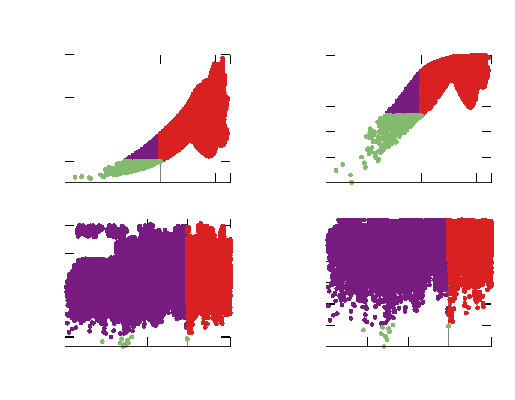
\includegraphics{./figures/h_and_h_not_fig}}%
    \gplfronttext
  \end{picture}%
\endgroup

  \vspace{0.3cm}
  \caption{\small The $\psi$-field (left) and \texttt{r}-field (right) of a
           configuration where Observation \ref{obs:observation_o} may (top)
           and may not (bottom) be made for $\delta \leq \delta_0$. Bottom:
           in contrast to the top row, set $\mathcal{V}$ is empty of admissible
           pose estimates for $\delta < 4.5 \ (\text{m}^2 +
           \text{rad}^2)^{1/2}$. The effect is produced in environment
           WILLOWGARAGE (pose $\bm{p}_{i}^G$; subsection \ref{subsec:exp_b})
           due to (a) the repetition of the immediate environment of the sensor
           more than once in the given map, and (b) the non-panoramic angular
           range of the sensor}
  \vspace{-0.5cm}
  \label{fig:h_and_h_not_fig}
\end{figure}


%%%%%%%%%%%%%%%%%%%%%%%%%%%%%%%%%%%%%%%%%%%%%%%%%%%%%%%%%%%%%%%%%%%%%%%%%%%%%%%%
\section{Conclusions and Future Steps}
  \label{section:finale}
  This article has presented a single-shot Monte Carlo approach to the solution
of the passive version of the global localisation problem with the use of a 2D
LIDAR sensor, titled CBGL. CBGL allows for the fast estimation of the sensor's
pose within a metric map by first dispersing hypotheses in it and then
leveraging (a) the proportionality of values of the Cumulative Absolute Error
per Ray (CAER) metric to the position and orientation errors of the hypotheses,
for estimates in a neighbourhood of the sensor's pose, and (b) the lack of
disproportionality outside of it. CBGL was evaluated in various real and
simulated conditions and environments; it was found to be superior to Monte
Carlo and feature-based approaches in terms of number of inlier pose estimates
and execution time. Future steps will aim at (a) the extension of the CAER
metric for the use with 3D LIDAR sensors in service to a solution of the
problem of their localisation in 6DoF, and (b) making CBGL more robust by
considering the statistics of clusters in case of disparate estimates in its
$\mathcal{H}_2$ set. The C++ ROS code of the proposed method is available at
\url{https://github.com/li9i/cbgl}.


%%%%%%%%%%%%%%%%%%%%%%%%%%%%%%%%%%%%%%%%%%%%%%%%%%%%%%%%%%%%%%%%%%%%%%%%%%%%%%%%
%\begin{thebibliography}{99}
  %\input{./sections/bibliography_ieee.bib}
%\end{thebibliography}

\bibliographystyle{ieeetran}
\bibliography{./sections/bibliography_ieee}

%%%%%%%%%%%%%%%%%%%%%%%%%%%%%%%%%%%%%%%%%%%%%%%%%%%%%%%%%%%%%%%%%%%%%%%%%%%%%%%%
% This command serves to balance the column lengths
% on the last page of the document manually. It shortens
% the textheight of the last page by a suitable amount.
% This command does not take effect until the next page
% so it should come on the page before the last. Make
% sure that you do not shorten the textheight too much.
%\addtolength{\textheight}{-1cm}

\balance

\end{document}
